\chapter{Géométrie\\dans l'espace} \label{G12}

\bigskip

\begin{figure}[h]
   \centering
      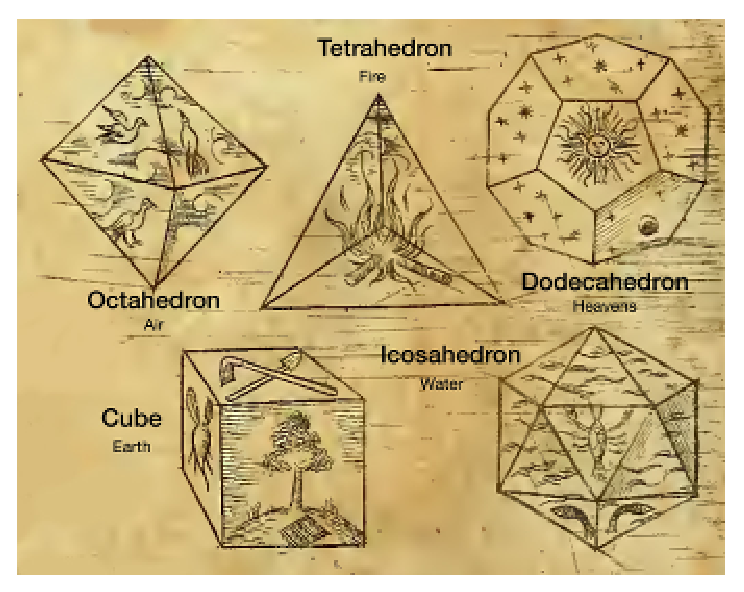
\includegraphics[height=6cm]{Geometrie/Images/G12_intro_Platon}
   \caption{Les solides de Platon, Harmonices Mundi, 1619 - Johannes Kepler}
\end{figure}

\bigskip

\begin{prerequis}[Un peu d'histoire]
   Les solides de l'espace figurent dans les livres 11 à 13 des {\it éléments} d'{\bf Euclide}. \\
   Parmi les solides de l'espace, il en est une sorte qui a été étudiée (entre autre) par le philosophe grec \textbf{Platon} ($-425$ ; $-348$ av. J.-C.) : les polyèdres réguliers et convexes. Dans le \textit{Timée}, l'un des derniers dialogues de Platon, ce dernier décrit la genèse du monde physique et de l'homme. Il associe chacun des quatre éléments physiques avec un solide régulier :      
  \begin{itemize}
      \item la Terre est associée avec le \textit{cube} : ces petits solides font de la poussière lorsqu'ils sont émiettés et se cassent lorsqu'on s'en saisit ;
      \item l'air avec l'\textit{octaèdre} : ses composants minuscules sont si doux qu'on peut à peine les sentir ;
      \item l'Eau avec l'\textit{icosaèdre} : elle s'échappe de la main lorsqu'on la saisit comme si elle était constituée de petites boules minuscules ;
      \item le feu avec le \textit{tétraèdre} : la chaleur du feu est pointue.    
   \end{itemize}
   Pour le cinquième solide, le \textit{dodécaèdre}, Platon le met en correspondance avec le tout, parce que c'est le solide qui ressemble le plus à la sphère.
\end{prerequis}

\cours

%%%%%%%%%
\section{Classification des solides} %%%%%1A

\subsection{Les polyèdres} %

\begin{definition}[Polyèdre]
   Un {\bf polyèdre} (de poly- plusieurs et -èdre face) est un solide de l'espace délimité par un nombre fini de polygones, appelés {\bf faces} du polyèdre. L'intersection de deux plans forment une {\bf arête} et ses extrémités sont appelés {\bf sommets} du polyèdre.
\end{definition}

{\psset{unit=0.6}
\begin{pspicture}(-0.5,-0.5)(25,6.5)
   \rput(3,3){%dodécaèdre
      \psSolid[object=dodecahedron,a=0.7,RotZ=50,action=draw**, fillcolor=A1!80]}
   \rput(7,2){%escalier
      \psSolid[object=new,sommets=
         0 0 0 %0
         1 0 0 %1
         1 1 0 %2
         1 1 0.5  %3
         0.5 1 0.5 %4
         0.5 1 1 %5
         0 1 1 %6
         0 0 1 %7
         0.5 0 0.5 %8
         1 0 0.5 %9
         0.5 0 1 %10
         0 1 0, %11
         faces={[0 1 9 8 10 7] [2 3 4 5 6 11] [1 2 3 9] [8 9 3 4] [4 5 10 8] [7 10 5 6] [0 7 6 11]},RotX=0,RotY=0,RotZ=100,action=draw**,fillcolor=A1!80]}
   \rput(16.2,2){%cône
      \psSolid[h=1.5,r=0.5,object=cone,ngrid=10 20,fillcolor=B1!70,action=draw**]}
   \rput(22,3){%tore
      \psSolid[r1=0.6,r0=0.3,object=tore,ngrid=15 20,fillcolor=B1!70,action=draw**]}
   \rput(6,0.3){\textcolor{A1}{polyèdres}}
   \rput(19,0.3){\textcolor{B1}{non polyèdres}}
\end{pspicture}}

Le nom des polyèdres est formé d'un préfixe qualifiant le nombre de faces suivi du siffixe -èdre. Par exemple : \medskip

{\hautab{1.2}
\begin{ltableau}{\linewidth}{8}
   \hline
   4 & 5 & 6 & 7 & 8 & 10 & 12 & 20 \\
   \hline
   tétraèdre & pentaèdre & hexaèdre & heptaèdre & octaèdre  & décaèdre & dodécaèdre & icosaèdre \\
   \hline
\end{ltableau} 
\vspace*{-2mm}
\begin{ltableau}{\linewidth}{4}
   \hline
   17 & 23 & 486 & 1\,000\;000 \\
   \hline
   heptadécaèdre & triaicosaèdre & hexaoctacontétrahectaèdre & mégaèdre \\
   \hline
\end{ltableau}}

\begin{pspicture}(0,-0.75)(16,2.5)
   \rput(2,1){\psSolid[object=tetrahedron,r=0.5,RotZ=20,fillcolor=yellow,action=draw*]}
   \rput(2,-0.6){4 faces}
   \rput(6,0.2){\psSolid[object=prisme,base=
-0.3 -0.3 0.3 -0.3 0 0.3,action=draw*,fillcolor=yellow!70,h=0.5]}
   \rput(6,-0.6){5 faces}
   \rput(10,1){\psSolid[object=cube,a=0.5,action=draw*,RotZ=20,fillcolor=yellow!40]}
   \rput(10,-0.6){6 faces}
   \rput(14,1){\psSolid[object=dodecahedron,a=0.4,RotZ=80,action=draw*, fillcolor=yellow!10]}
   \rput(14,-0.6){12 faces}
\end{pspicture}


\subsection{Convexité} %

\begin{definition}[Convexité]
   Un solide est {\bf convexe} si, lorsque l'on prend deux points quelconques du solide, le segment tout entier joignant ces deux points reste à l'intérieur du solide.
\end{definition}

{\psset{unit=0.6}
\begin{pspicture}(-0.5,0.6)(25,6.5)
   \rput(3,3){%dodécaèdre
      \psSolid[object=dodecahedron,a=0.7,RotZ=50,action=draw**, fillcolor=A1!80]}
   \rput(8.7,2){%cône
      \psSolid[h=1.5,r=0.5,object=cone,ngrid=10 20,fillcolor=A1!80,action=draw**]}
   \rput(14,2){%escalier
      \psSolid[object=new,sommets=
         0 0 0 %0
         1 0 0 %1
         1 1 0 %2
         1 1 0.5  %3
         0.5 1 0.5 %4
         0.5 1 1 %5
         0 1 1 %6
         0 0 1 %7
         0.5 0 0.5 %8
         1 0 0.5 %9
         0.5 0 1 %10
         0 1 0, %11
         faces={[0 1 9 8 10 7] [2 3 4 5 6 11] [1 2 3 9] [8 9 3 4] [4 5 10 8] [7 10 5 6] [0 7 6 11]},RotX=0,RotY=0,RotZ=100,action=draw**,fillcolor=B1!70]} 
   \rput(22,3.5){%tore
      \psSolid[r1=0.6,r0=0.3,object=tore,ngrid=15 20,fillcolor=B1!70,action=draw**]}
   \rput(6,0.3){\textcolor{A1}{solides convexes}}
   \rput(19,0.3){\textcolor{B1}{solides non convexes}}
\end{pspicture}}


\section{Représentations des solides} %%%%% B

\subsection{Perspective cavalière} 

Pour représenter un solide de l'espace, on peut utiliser la {\bf perspective cavalière} : technique de dessin permettant de représenter un solide sur une surface à deux dimensions dans lequel le parallélisme et les proportions sur les arêtes sont respectés, et où les angles ne sont respectés que dans les face de devant et du fond.

\begin{methode}[Représenter un solide en perspective cavalière]
   Pour représenter un solide en perspective cavalière :
   \begin{enumerate}
      \item on trace en vraie grandeur la face de devant ;
     \item on trace les arêtes visibles des faces latérales parallèles et de même longueur : ce sont les fuyantes, plus courtes que leur mesure réelle ;
      \item on trace les arêtes cachées en pointillés.
   \end{enumerate}
   \exercice
      {\psset{unit=0.85}
      \begin{pspicture}(-1,-0.5)(5,3.7)
         \pspolygon(0,0)(4,0)(5,1)(5,3)(1,3)(0,2)
         \psline(0,2)(4,2)(4,0)
         \psline(4,2)(5,3)
         \psline[linestyle=dashed](0,0)(1,1)(5,1)
         \psline[linestyle=dashed](1,1)(1,3)
         \rput(0,-0.3){$A$}
         \rput(4,-0.3){$B$}
         \rput(5.1,0.7){$C$}
         \rput(1.2,0.7){$D$}
         \rput(0,2.3){$E$}
         \rput(4,2.3){$F$}
         \rput(5,3.3){$G$}
         \rput(1,3.3){$H$}
      \end{pspicture}}
   \correction
      Ce parallélépipède rectangle possède :
      \begin{itemize}
         \item 8 \textbf{sommets} : $A, B, C, D, E, F, G$ et $H$ ;
         \item 12 \textbf{arêtes} : $[AB], [BC], [AE], [BF], [EF], [FG], [CG], [EH]$ et $[GH]$ apparentes, et $[AD], [DC]$ et $[DH]$ cachées ;
         \item 6 \textbf{faces} : $ABFE$ est la face de devant, $CDHG$ celle de derrière, $ABCD$ la face du dessous, $EFGH$ celle du dessus, $BCGF$ la face de droite, et $ADHE$ celle de gauche.
      \end{itemize}
\end{methode}

\medskip

\subsection{Différentes vues} %

On peut représenter un solide par ses différentes vues : de face, de derrière, de côté (droite et gauche) , de dessus, de dessous.

\begin{center}
   {\psset{unit=0.9}
   \begin{pspicture}(0,0)(17,9.5)
      %pièces centrale
      \pspolygon[fillstyle=solid,fillcolor=yellow!50](6.5,3.5)(8,3.5)(8,3)(9,3)(10,4)(10,5)(10.5,5.5)(10.5,6.5)(10,6.5)(10,7)(9,7)(8.5,6.5)(8.5,6)(8,6)(7.5,5.5)(7.5,5)(7,5)(6.5,4.5)
      \psline(6.5,4.5)(7.5,4.5)(7.5,5.5)(8.5,5.5)(8.5,6.5)(9.5,6.5)(9.5,4.5)(9,4)(8,4)(8,3.5)
      \psline(9,3)(9,4)
      \psline(8,4)(8.5,4.5)(9.5,4.5)
      \psline(9.5,6.5)(10,7)(10,6)(10.5,6.5)   
      %gauche
      \pspolygon[fillstyle=solid,fillcolor=yellow!20](0,5)(0,6)(1,6)(1,7)(2,7)(2,5)(3,5)(3,4)(1,4)(1,5)
      \psline(2,4)(2,5)(1,5)(1,6)(2,6)
      \psline[arrowsize=0.5]{->}(3.5,5)(6,5)
      \rput(1.5,3.5){vue de gauche}
      %face
      \pspolygon[fillstyle=solid,fillcolor=yellow!10](2,0)(5,0)(5,3)(4,3)(4,2)(3,2)(3,1)(2,1)
      \psline(4,0)(4,1)(5,1)
      \psline[arrowsize=0.5]{->}(5.5,1.5)(7,3)
      \rput(3.5,-0.5){vue de face}
      %dessous
      \pspolygon[fillstyle=solid,fillcolor=yellow!10](10,1)(12,1)(12,0)(13,0)(13,3)(12,3)(12,2)(10,2)
      \psline(12,2)(13,2)
      \psline[arrowsize=0.5]{->}(9.5,1.5)(8.5,1.5)(8.5,2.5)
      \rput(11.5,-0.5){vue de dessous}
      %droite
      \pspolygon[fillstyle=solid,fillcolor=yellow!10](14,4)(16,4)(16,5)(17,5)(17,6)(16,6)(16,7)(15,7)(15,5)(14,5)
      \psline[arrowsize=0.5]{->}(13,5)(11,5)
      \rput(15.5,3.5){vue de droite}
      %derriere
      \pspolygon[fillstyle=solid,fillcolor=yellow!10](11,7)(14,7)(14,8)(13,8)(13,9)(12,9)(12,10)(11,10)
      \psline(11,8)(12,8)(12,9)(11,9)
      \psline[arrowsize=0.5]{->}(10.5,9)(9.5,7.5)
      \rput(12.5,6.5){vue de derrière}
      %dessus
      \pspolygon[fillstyle=solid,fillcolor=yellow!10](6,7)(6,10)(5,10)(5,9)(3,9)(3,8)(5,8)(5,7)
      \psline(6,9)(5,9)(5,8)(6,8)
      \psline(4,8)(4,9)
      \psline[arrowsize=0.5]{->}(6.5,8.5)(8,8.5)(8,7)
      \rput(4.5,6.5){vue du dessus}
   \end{pspicture}}
\end{center}


\subsection{Patrons} %

\begin{definition}[Patron]
   Le \textbf{patron} d'un solide est une surface plane d'un seul tenant qui, par pliage, permet de reconstituer le solide sans recouvrement de ses faces. \smallskip
\end{definition}

\medskip

Un patron se dessine en dépliant mentalement le solide.

\begin{exemple}  
   {\psset{fillstyle=solid,unit=0.45}
   \begin{pspicture}(-7,-4)(5,6.)  
      \pspolygon[fillcolor=A2](-5.38,-3.26)(-1.46,-3.74)(-2.88,-1.66)(-6.74,-1.04)
\pspolygon[fillcolor=yellow!50](-1.06,-1.36)(4.36,0.74)(3.94,-1.66)(-1.46,-3.74)
\pspolygon[fillcolor=B2](-6.54,-0.46)(-5.24,3.82)(0.12,5.9)(-1.22,1.66)
\pspolygon[fillcolor=A2](4.48,1.22)(0.64,1.82)(0.12,-0.90)(4.36,0.74)
\pspolygon[fillcolor=yellow!50](0.12,-0.90)(-1.22,1.66)(-6.54,-0.46)(-6.27,-1.12)(-2.88,-1.66)(-2.55,-2.15)(-1.11,-1.68)(-1.06,-1.36)
\pspolygon[fillcolor=B2](-1.46,-3.74)(-2.55,-2.15)(-1.11,-1.68)
   \end{pspicture}}
\correction
   {\psset{fillstyle=solid}
   \begin{pspicture}(-2,0)(6,4.25)
      \psframe[fillcolor=B2](-1,1)(1,3.5)
      \psframe[fillcolor=yellow!50](1,1)(2,3.5)
      \psframe[fillcolor=B2](2,1)(4,3.5)
      \psframe[fillcolor=yellow!50](4,1)(5,3.5)
      \psframe[fillcolor=A2](2,3.5)(4,4.5)
      \psframe[fillcolor=A2](2,1)(4,0)
   \end{pspicture}}
\end{exemple}

\medskip

Le patron d'un polyèdre n'est pas unique, il dépend de la manière dont on le déplie. On sera vigilant à bien vérifier la cohérence des mesures pour que le patron se referme bien.

{\psset{unit=0.75}
\begin{pspicture}(-4.5,0.2)(6,5)
   \psline(1,0)(1,1)(0,1)(0,3.5)(1,3.5)(1,4.5)(3,4.5)(3,3.5)(4,3.5)(6,3.5)(6,1)(4,1)(3,1)(3,0)(1,0)
   \psframe(1,1)(3,3.5)
   \psline(4,3.5)(4,1)
   \rput(0.5,1){\textcolor{B2}{x}}
   \rput(1,0.5){\textcolor{B2}{x}}
   \rput(0.5,3.5){\textcolor{B2}{x}}
   \rput(1,4){\textcolor{B2}{x}}
   \rput(3.5,1){\textcolor{B2}{x}}
   \rput(3,0.5){\textcolor{B2}{x}}
   \rput(3.5,3.5){\textcolor{B2}{x}}
   \rput(3,4){\textcolor{B2}{x}}
   \rput(0,2.25){\textcolor{A1}{o}}
   \rput(1,2.25){\textcolor{A1}{o}}
   \rput(3,2.25){\textcolor{A1}{o}}
   \rput(4,2.25){\textcolor{A1}{o}}
   \rput(6,2.25){\textcolor{A1}{o}}
   \rput(2,0){\textcolor{G1}{||}}
   \rput(2,1){\textcolor{G1}{||}}
   \rput(2,3.5){\textcolor{G1}{||}}
   \rput(2,4.5){\textcolor{G1}{||}}
   \rput(5,1){\textcolor{G1}{||}}
   \rput(5,3.5){\textcolor{G1}{||}}
   \rput(2,2.5){\it pavé}
   \rput(2,2){\small\it droit}
\end{pspicture}}
\begin{pspicture}(-5,-0.5)(4,3)
   \pspolygon(1,0)(1,1)(-1,1)(-1,2)(1,2)(1,3)(2,3)(2,2)(3,2)(3,1)(2,1)(2,0)(1,0)(1,1)   
   \psframe(1,1)(2,2)
   \psline(0,1)(0,2)
   \rput(0,1.5){\textcolor{B2}{x}}
   \rput(0.5,1){\textcolor{B2}{x}}
   \rput(0.5,2){\textcolor{B2}{x}}
   \rput(1,0.5){\textcolor{B2}{x}}
   \rput(1,2.5){\textcolor{B2}{x}}
   \rput(1.5,0){\textcolor{B2}{x}}
   \rput(1.5,3){\textcolor{B2}{x}}
   \rput(2.5,1){\textcolor{B2}{x}}
   \rput(2.5,2){\textcolor{B2}{x}}
   \rput(-0.5,1){\textcolor{B2}{x}}
   \rput(-0.5,2){\textcolor{B2}{x}}
   \rput(2,0.5){\textcolor{B2}{x}}
   \rput(2,1.5){\textcolor{B2}{x}}
   \rput(2,2.5){\textcolor{B2}{x}}
   \rput(3,1.5){\textcolor{B2}{x}}
   \rput(1,1.5){\textcolor{B2}{x}}
   \rput(-1,1.5){\textcolor{B2}{x}}
   \rput(1.5,1.5){\small\it cube}
\end{pspicture}

{\psset{unit=0.9}
\begin{pspicture}(0,-0.5)(6,2)
   \psframe(1,-0.1)(5,3)
   \pspolygon(1,1)(5,1)(5.85,1.6)(5,2)(1,2)(0.15,1.6)
   \rput(3,-0.1){\textcolor{B2}{x}}
   \rput(3,1){\textcolor{B2}{x}}
   \rput(3,2){\textcolor{B2}{x}}
   \rput(3,3){\textcolor{B2}{x}}
   \rput(1,0.45){\textcolor{blue}{*}}
   \rput(1,1.5){\textcolor{J1}{=}}
   \rput(1,2.5){\textcolor{A1}{o}}
   \rput(5,0.45){\textcolor{blue}{*}}
   \rput(5,1.5){\textcolor{J1}{=}}
   \rput(5,2.5){\textcolor{A1}{o}}
   \rput(0.55,1.27){\textcolor{blue}{*}}
   \rput(0.55,1.77){\textcolor{A1}{o}}
   \rput(5.45,1.27){\textcolor{blue}{*}}
   \rput(5.45,1.77){\textcolor{A1}{o}}
   \rput(3,1.5){\small\it prisme droit}
\end{pspicture}
\begin{pspicture}(-6,-2.7)(2,2)
   \psframe(-1,-1)(1,1)
   \pspolygon(-2.5,0)(-1,-1)(0,-2.5)(1,-1)(2.5,0)(1,1)(0,2.5)(-1,1)
   \rput(0,-1){\textcolor{B2}{x}}
   \rput(0,1){\textcolor{B2}{x}}
   \rput(-1,0){\textcolor{B2}{x}}
   \rput(1,0){\textcolor{B2}{x}}      
   \rput(-1.75,-0.5){\textcolor{A1}{o}}
   \rput(-1.75,0.5){\textcolor{A1}{o}}
   \rput(1.75,-0.5){\textcolor{A1}{o}}
   \rput(1.75,0.5){\textcolor{A1}{o}}
   \rput(-0.5,1.75){\textcolor{A1}{o}}
   \rput(-0.5,1.75){\textcolor{A1}{o}}
   \rput(0.5,-1.75){\textcolor{A1}{o}}
   \rput(-0.5,-1.75){\textcolor{A1}{o}}
   \rput(0.5,1.75){\textcolor{A1}{o}}
   \rput(0,0.2){\small\it pyramide}
   \rput(0,-0.2){\small\it régulière}
\end{pspicture}

Pour les solide qui ne sont pas polyédriques, on parle de plutôt de développement. \\
\begin{pspicture}(-8,-2)(2,2.5)
   \psframe(-2,-1)(2,1)
   \pscircle(0,1.64){0.64}
   \pscircle(0,-1.64){0.64}
   \rput(-2,0){\textcolor{B2}{x}}
   \rput(2,0){\textcolor{B2}{x}}
   \rput(0,-1){\textcolor{A1}{o}}
   \rput(0,1){\textcolor{A1}{o}}
   \rput(0,0){\small\it cylindre de révolution}
\end{pspicture}
\begin{pspicture}(-6,-2)(3,2.5)
   \pscircle(-1.75,0){0.75}
   \pswedge(2,0){3}{130}{230}
   \rput(0.25,0.2){\small\it cône de}
   \rput(0.25,-0.2){\small\it révolution}
\end{pspicture}}


\subsection{Sections de solides} %%

\begin{propriete}[Section d'un pavé droit]
   \begin{itemize}
      \item La section d'un pavé droit par un plan parallèle à une des faces est un rectangle de mêmes dimension que cette face.
      \item La section d'un pavé droit par un plan parallèle à une arête est un rectangle. \\ [-8mm]
   \end{itemize}
\end{propriete}

\begin{propriete}[Section d'une sphère]
   La section d'une sphère par un plan est un cercle.
\end{propriete}

\begin{propriete}[Section d'un cylindre]
   \begin{itemize}
      \item La section d'un cylindre de révolution par est un plan parallèle à l'une de ses bases est un cercle de même rayon que la base.
      \item La section d'un cylindre de révolution par est un plan parallèle à l'axe de révolution est un rectangle. \\ [-8mm]
   \end{itemize}
\end{propriete}

\begin{propriete}[Section d'un cône ou d'une pyramide]
   La section d'une pyramide ou d'un cône cylindre de révolution par est un plan parallèle à la base est une réduction de la base de la pyramide ou du cône.
\end{propriete}

\begin{center}
   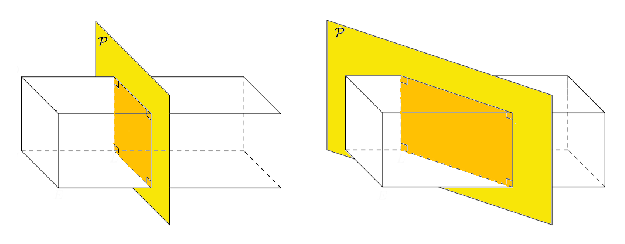
\includegraphics[height=4cm]{Geometrie/Images/G12_cours_section_pave} \qquad
   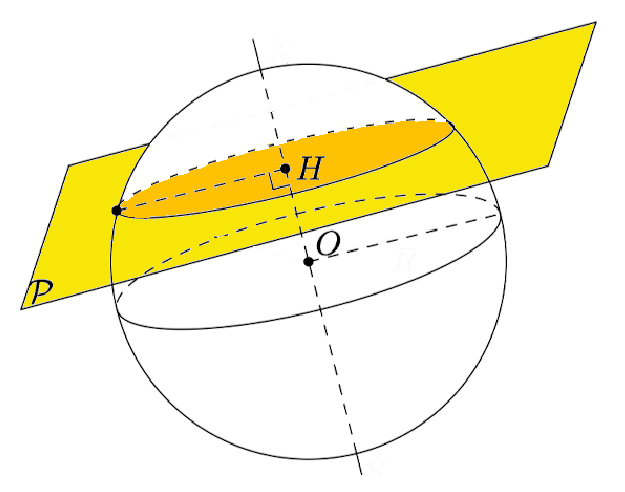
\includegraphics[height=3.5cm]{Geometrie/Images/G12_cours_section_sphere} \\ [5mm]
   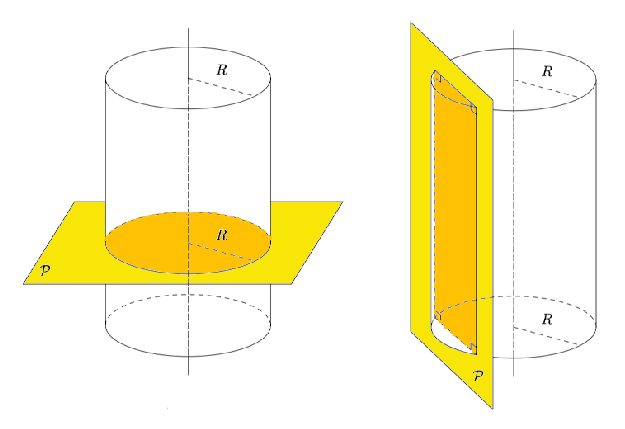
\includegraphics[height=5.3cm]{Geometrie/Images/G12_cours_section_cylindre} \qquad
   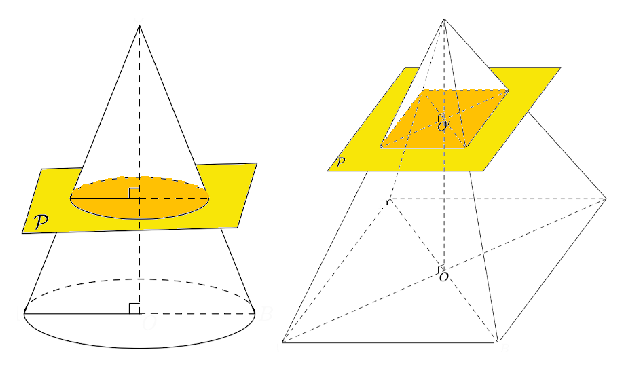
\includegraphics[height=4.5cm]{Geometrie/Images/G12_cours_section_cone_pyramide}
\end{center}

\pagebreak

\section{Solides usuels} %%%3

\begin{center}
{\hautab{1.5}
\begin{CLtableau}{0.93\linewidth}{3}{C{1.8}|C{4.5}|C{8}}
   \hline
   nom & représentation & propriétés \\
   \hline
   \begin{minipage}{3cm}
      cube
   \end{minipage} & 
   \begin{minipage}{5cm}
      {\psset{unit=0.8}
      \begin{pspicture}(-1,-0.5)(3,3.5)
         \pspolygon(0,0)(2,0)(3,1)(3,3)(1,3)(0,2)
         \psline(0,2)(2,2)(2,0)
         \psline(2,2)(3,3)
         \psline[linestyle=dashed](0,0)(1,1)(3,1)
         \psline[linestyle=dashed](1,1)(1,3)
      \end{pspicture}}
   \end{minipage} &
   \begin{minipage}{7.5cm}
      un cube est un polyèdre possédant 6 faces qui sont des carrés
   \end{minipage} \\
   \hline
   \begin{minipage}{3cm}
      pavé
   \end{minipage}
   & 
   \begin{minipage}{5cm}
   {\psset{xunit=0.7,yunit=0.6}
         \begin{pspicture}(-0.5,-0.75)(5,3.75)
         \pspolygon(0,0)(4,0)(5,1)(5,3)(1,3)(0,2)
         \psline(0,2)(4,2)(4,0)
         \psline(4,2)(5,3)
         \psline[linestyle=dashed](0,0)(1,1)(5,1)
         \psline[linestyle=dashed](1,1)(1,3)
      \end{pspicture}}
   \end{minipage}
   & 
   \begin{minipage}{7.5cm}
      un pavé, ou parallélépipède rectangle est un polyèdre possédant 6 faces qui sont des rectangles
   \end{minipage} \\
   \hline
   \begin{minipage}{3cm}
      prisme
   \end{minipage}
   &
   \begin{minipage}{5cm}
      {\psset{xunit=0.6,yunit=0.5}
      \begin{pspicture}(-1,-1.5)(5,3.75)         
         \pspolygon(0,0)(2,-1)(4,0)(5,1)(5,3)(1,3)(0,2)
         \psline(0,2)(2,1)(4,2)(4,0)
         \psline(4,2)(5,3)
         \psline[linestyle=dashed](0,0)(1,1)(5,1)
         \psline[linestyle=dashed](1,1)(1,3)
         \psline(2,-1)(2,1)
      \end{pspicture}}
   \end{minipage}
   &
   \begin{minipage}{7.5cm}
      un prisme est un polyèdre possédant deux faces polygonales parallèles et isométriques, les autres étant des rectangles
   \end{minipage} \\
   \hline
   \begin{minipage}{3cm}
      pyramide
   \end{minipage}
   &
   \begin{minipage}{5cm}
      {\psset{yunit=0.3,xunit=0.7}
      \begin{pspicture}(-0.5,-1.25)(5,7)         
         \pspolygon(1,0)(4,0)(5,1)(2.5,6)(0,1)
         \psline(1,0)(2.5,6)(4,0)
         \psline[linestyle=dashed](0,1)(1.3,2)(3.7,2)(5,1)
         \psline[linestyle=dashed](1.3,2)(2.5,6)(3.7,2)
      \end{pspicture}}
   \end{minipage}
   &
   \begin{minipage}{7.5cm}
      une pyramide est un polyèdre dont la base est un polygone et dont toutes les autres faces sont des triangles ayant un sommet commun appelé sommet de la pyramide
  \end{minipage} \\
  \hline
  \begin{minipage}{3cm}
      cylindre
   \end{minipage}
   &
   \begin{minipage}{5cm}
      {\psset{xunit=0.7,yunit=0.4}
      \begin{pspicture}(-1,-0.75)(5,6.75)       
         \psline(4,1)(4,5)
         \psline(0,1)(0,5)
         \psellipse(2,5)(2,1)
         \psellipticarc(2,1)(2,1){180}{0}
         \psellipticarc[linestyle=dashed](2,1)(2,1){0}{180}
      \end{pspicture}}
   \end{minipage}
   &
   \begin{minipage}{7.5cm}
      un cylindre (de révolution) est un solide à deux faces parallèles en forme de disque de même rayon et dont la surface latérale est engendrée par le déplacement d'une droite orthogonale au disque et suivant le contour de ce disque
  \end{minipage} \\
  \hline
  \begin{minipage}{3cm}
      cône
   \end{minipage}
   &
   \begin{minipage}{3cm}
       {\psset{yunit=0.4,xunit=0.8}
       \begin{pspicture}(0,-1)(5,7)       
         \psline(4,1)(2,6)(0,1)
         \psellipticarc(2,1)(2,1){180}{0}
         \psellipticarc[linestyle=dashed](2,1)(2,1){0}{180}
      \end{pspicture}}
   \end{minipage}
   &
   \begin{minipage}{7.5cm}
      un cône (de révolution) est un solide à une face en forme de disque et dont la surface latérale est engendrée par le déplacement d'une droite qui décrit la circonférence du disque autour d'un point fixe appelé le sommet du cône  
   \end{minipage} \\
   \hline
   \begin{minipage}{3cm}
      sphère
   \end{minipage}
   &
   \begin{minipage}{5cm}
      {\psset{unit=0.5}
      \begin{pspicture}(-1.75,-0.75)(3.5,5.75)         
         \pscircle(2.5,2.5){2.5}
         \psellipticarc[linestyle=dashed](2.5,2.5)(2.5,1){0}{180}
         \psellipticarc(2.5,2.5)(2.5,1){180}{0}
         \rput(2.5,2){$O$}
         \psdot(2.5,2.5)
      \end{pspicture}}
   \end{minipage} 
   &
   \begin{minipage}{7.5cm}
      une sphère de centre O et de rayon $r$ est l'ensemble des points $M$ de l'espace tels que $OM=r$
   \end{minipage} \\
   \hline
\end{CLtableau}}
\end{center}  


\section{Positions relatives de droites et de plans} %%%%% D

On rappelle les propriétés suivantes : \\
-- Par deux points distincts $A$ et $B$ de l'espace passe une seule droite, notée $(AB)$. \\
-- Par trois points non alignés $A, B$ et $C$ de l'espace passe un seul plan, noté $(ABC)$. \\
-- Si un plan contient deux points $A$ et $B$, alors il contient toute la droite $(AB)$. \\
-- Dans tout plan de l’espace, tout résultat de géométrie plane s’applique. \medskip

\subsection{Orthogonalité} %

\begin{definition}[Droite(s) orthogonale(s)]
   \begin{itemize}
      \item Deux droites de l’espace sont {\bf orthogonales} si leurs parallèles menées par un point sont perpendiculaires.
      \item Une droite est {\bf orthogonale} à un plan si elle est perpendiculaire à deux droites sécantes de ce plan. \\ [-8mm]
   \end{itemize}
\end{definition}

\smallskip

\begin{propriete}[Orthogonalité d'une droite par rapport à un plan]
   Si une droite est perpendiculaire à deux droites sécantes du plan, alors elle est orthogonale au plan (et donc à toute droite du plan). \smallskip
\end{propriete}

\begin{center}
   \begin{pspicture}(0,-0.5)(5,3)
      \pspolygon(0,0)(4,0)(5,2)(1,2)  
      \rput(0.5,0.3){$\mathcal{P}$}
      \psline[linecolor=B1](2.5,1)(2.5,3)
      \psline[linecolor=B1, linestyle=dashed](2.5,0.9)(2.5,-0.1)
      \psline[linecolor=B1](2.5,0)(2.5,-0.5)
      \psline[linecolor=A1](1,0.5)(4,1.5)
      \psline[linecolor=A1](1.5,1.5)(3.5,0.5)
      \psline[linecolor=B1](2.5,1.2)(2.65,1.1)(2.65,0.92)
      \psline[linecolor=B1](2.5,1.2)(2.7,1.3)(2.7,1.05)
   \end{pspicture}
\end{center}

\begin{remarques}
   \begin{itemize}
      \item Un plan est une surface plane illimitée. Il est entièrement déterminé par trois points non alignés. Cette surface est représentée en perspective par un parallélogramme.
      \item Dans l’espace, des droites orthogonales ne sont pas nécessairement coplanaires (situées dans un même plan) et n’ont donc pas nécessairement de point d’intersection. \\
   \end{itemize}
\end{remarques}

\begin{exemple}
 $ABCDEFGH$ est un pavé droit.
   \begin{center}
   \begin{pspicture}(0,-1)(5,3.2)
      {\psset{xunit=1.5,yunit=0.9}
      \pspolygon(0,0)(2,0)(3,1)(3,3)(1,3)(0,2)
      \psline(0,2)(2,2)(2,0)
      \psline(2,2)(3,3)         
      \psline[linestyle=dashed](0,0)(1,1)(3,1)
      \psline[linestyle=dashed](1,1)(1,3)
      \rput(-0.2,-0.2){$A$}
      \rput(2,-0.3){$B$}
      \rput(2.2,1.8){$F$}
      \rput(-0.2,2){$E$}
      \rput(0.8,1.2){$D$}
      \rput(3.2,1){$C$}
      \rput(3.1,3.3){$G$}
      \rput(1,3.4){$H$}}
   \end{pspicture}
   \end{center}
\correction
   \ \\ [-9mm]
   \begin{itemize}
      \item La face $EFGH$ du dessus est contenue dans le plan $(EHG)$, ou $(EFG)$, ou $(HEF)$\dots{} il suffit de choisir trois points non alignés de la face.
      \item Les droites $(EA)$ et $(FG)$ sont orthogonales car $(EA)$ est perpendiculaire à $(EH)$, elle même parallèle à $(FG)$. 
      \item La droite $(CB)$ est orthogonale au plan $(ABF)$ puisque $(CB)$ est perpendiculaire à $(BA)$ et à $(BF)$ qui sont deux droites sécantes du plan $(ABF)$.
   \end{itemize}
\end{exemple}

\pagebreak
\subsection{Positions relatives} %

\textbf{Position relative de deux droites}

{\psset{yunit=0.7}
\begin{minipage}{6cm}
   \begin{center} 
      Droites coplanaires sécantes : \\
      un point d'intersection
      \begin{pspicture}(6,3.9)
         \pspolygon(0,0)(4,0)(5,3)(1,3)  
         \psline[linecolor=B2](0.5,0)(4,3)
         \rput(1.4,0.3){\textcolor{B2}{$d_1$}}
         \psline[linecolor=A1](0.75,2.25)(4.25,0.75)
         \rput(4.1,1.3){\textcolor{A1}{$d_2$}}
         \psdot[dotstyle=+,dotscale=2](2.35,1.55)
         \rput(2.4,2){$A$}
      \end{pspicture}
   \end{center}
\end{minipage}
\begin{minipage}{6cm}
   \begin{center} 
      Droites coplanaires parallèles : \\
      aucun ou une infinité de points d'intersection
      \begin{pspicture}(6,3.5)
         \pspolygon(0,0)(4,0)(5,3)(1,3)  
         \psline[linecolor=B2](0.5,0)(4,3)
         \rput(1.8,2){\textcolor{B2}{$d_1=d_3$}}
         \psline[linecolor=A1](1.5,0)(5,3)
         \rput(3,0.8){\textcolor{A1}{$d_2$}}
      \end{pspicture}
   \end{center}
\end{minipage}
\begin{minipage}{6cm}
   \begin{center} 
      Droites non coplanaires : \\
      aucun point d'intersection
      \begin{pspicture}(6,3.9)
         \pspolygon(0,0)(4,0)(5,3)(1,3)  
         \psline[linecolor=B2](0.5,0)(4,3)
         \rput(1.4,0.3){\textcolor{B2}{$d_1$}}
         \psline[linecolor=A1](1,3.3)(1.5,2.4)
         \psdot[dotstyle=+,dotscale=2,linecolor=A1](1.5,2.4)
         \psline[linecolor=A1, linestyle=dashed](1.5,2.4)(2.83,0)
         \psline[linecolor=A1](2.83,0)(3.5,-1.2)
         \rput(3.1,0.3){\textcolor{A1}{$d_2$}}
      \end{pspicture}
   \end{center}
\end{minipage}}

\smallskip

\textbf{Position relative de deux plans} 

{\psset{yunit=0.7}
\begin{minipage}{6cm}
   \begin{center} 
      Plans sécants : \\
      une droite d'intersection
      \begin{pspicture}(6,5)
         \psline[linecolor=A1](3.5,3)(5,3)(4,0)(0,0)(1,3)(1.5,3) 
         \psline[linecolor=A1,linestyle=dotted](1.5,3)(3.5,3)
         \rput(0.4,0.4){\textcolor{A1}{$\mathcal{P}_1$}}
         \psarc[linecolor=A1](0,0){0.8}{0}{63}
         \psline[linecolor=B2](3.17,0)(3,-0.5)(1,1.5)(2,4.5)(3.5,3)
         \psline[linecolor=B2,linestyle=dotted](3.5,3)(4,2.5)(3.17,0)
         \rput(2.1,3.9){\textcolor{B2}{$\mathcal{P}_2$}}
         \psarc[linecolor=B2](2,4.5){0.8}{-115}{-35}
         \psline(2.3,-0.5)(3.7,3.7)
         \rput(3.8,3.4){$d$}     
      \end{pspicture}
   \end{center}
\end{minipage}
\begin{minipage}{6cm}
   \begin{center} 
      Plans parallèles strictement:\\aucun point d'intersection
      \begin{pspicture}(6,5)
         \psline[linecolor=A1](0.35,1)(0,0)(4,0)(5,3)(4.7,3)
         \psline[linecolor=A1,linestyle=dotted](4.7,3)(1,3)(0.35,1)
         \rput(0.5,0.4){\textcolor{A1}{$\mathcal{P}_1$}}
         \psarc[linecolor=A1](0,0){0.8}{0}{63}
         \pspolygon[linecolor=B2](0,1)(4,1)(5,4)(1,4) 
         \rput(1.2,3.6){\textcolor{B2}{$\mathcal{P}_2$}}
         \psarc[linecolor=B2](1,4){0.6}{-115}{0}
      \end{pspicture}
   \end{center}
\end{minipage}
\begin{minipage}{6cm}
   \begin{center} 
      Plans parallèles confondus :\\un plan d'intersection
      \begin{pspicture}(6,5)
         \pspolygon(0,0)(4,0)(5,3)(1,3)  
         \rput(2.5,1.5){$\mathcal{P}_1=\mathcal{P}_2$}
      \end{pspicture}
   \end{center}
\end{minipage}}

\medskip

\textbf{Position relative d'une droite et d'un plan}

{\psset{yunit=0.7}
\begin{minipage}{6cm}
   \begin{center} 
      Droite et plan sécants :\\un point d'intersection
      \begin{pspicture}(6,4)
         \pspolygon[linecolor=A1](0,0)(4,0)(5,3)(1,3)  
         \rput(0.4,0.4){\textcolor{A1}{$\mathcal{P}_1$}}
         \psarc[linecolor=A1](0,0){0.8}{0}{63}
         \psline[linecolor=B2](1,3.3)(2,1.5)
         \psdot[dotstyle=+,dotscale=2](2,1.5)
         \rput(2.3,1.8){$A$}
         \psline[linecolor=B2](1,3.3)(1.5,2.4)
         \psline[linecolor=B2, linestyle=dashed](1.5,2.4)(2.83,0)
         \psline[linecolor=B2](2.83,0)(3.5,-1.2)
         \rput(3.1,0.4){\textcolor{B2}{$d$}}
      \end{pspicture}
   \end{center}
\end{minipage}
\begin{minipage}{6cm}
   \begin{center} 
      Droite et plan parallèles :\\droite incluse dans le plan
      \begin{pspicture}(6,4)
         \pspolygon[linecolor=A1](0,0)(4,0)(5,3)(1,3)  
         \rput(0.4,0.4){\textcolor{A1}{$\mathcal{P}_1$}}
         \psarc[linecolor=A1](0,0){0.8}{0}{63}
         \psline[linecolor=B2](0.8,0)(4,3)
         \rput(3,2.5){\textcolor{B2}{$d$}}
      \end{pspicture}
   \end{center}
\end{minipage}
\begin{minipage}{6cm}
   \begin{center} 
      Droite et plan parallèles :\\aucun point d'intersection
      \begin{pspicture}(6,4)
         \pspolygon[linecolor=A1](0,0)(4,0)(5,3)(1,3)  
         \psline[linecolor=B2](3,-0.5)(1,3.5)
         \rput(0.4,0.4){\textcolor{A1}{$\mathcal{P}_1$}}
         \psarc[linecolor=A1](0,0){0.8}{0}{63}
         \rput(2.6,-0.3){\textcolor{B2}{$d$}}
      \end{pspicture}
   \end{center}
\end{minipage}}

\bigskip

\begin{exemple}
   $ABCDEFGH$ est un pavé droit.
   \begin{center}
   \begin{pspicture}(0,-0.5)(5,3.5)
      {\psset{xunit=1.5}
      \pspolygon(0,0)(2,0)(3,1)(3,3)(1,3)(0,2)
      \psline(0,2)(2,2)(2,0)
      \psline(2,2)(3,3)         
      \psline[linestyle=dashed](0,0)(1,1)(3,1)
      \psline[linestyle=dashed](1,1)(1,3)
      \psdot(2.2,3)
      \rput(-0.2,-0.2){$A$}
      \rput(2,-0.3){$B$}
      \rput(2.3,3.4){$I$}
      \rput(2.2,1.8){$F$}
      \rput(-0.2,2){$E$}
      \rput(0.8,1.2){$D$}
      \rput(3.2,1){$C$}
      \rput(3.1,3.3){$G$}
      \rput(1,3.4){$H$}}
   \end{pspicture}
   \end{center}
\correction
   \ \\ [-10mm]
   \begin{itemize}
      \item Les droites $(IF)$ et $(EG)$ sont coplanaires et sécantes, elles définissent le plan $(HEF)$.
      \item Les droites $(HF)$ et $(DB)$ sont parallèles, elles définissent le plan $(DBF)$. 
      \item Les droites $(HE)$ et $(IC)$ sont non coplanaires.
      \item Les plans $(IFB)$et $(AEF)$ sont sécants suivant la droite (FB).
      \item Les plans $(DHC)$ et $(FBA)$ sont parallèles.
      \item Les droites $(HF)$ et $(AC)$ sont dans des plans parallèles, mais elles ne sont pas parallèles.
   \end{itemize}
\end{exemple}

\pagebreak

%%%%%%%%%%%%%%%%%%%%%%%%%%%%%%%%%
\section{Se représenter dans l'espace}

\subsection{Repérage sur un parallélépipède rectangle}

\begin{definition}[Repère dans un pavé]
   Dans un parallélépipède rectangle, un {\bf repère} est formé par trois arêtes ayant un sommet commun appelé origine du repère.
\end{definition}

\smallskip

\begin{propriete}[Coordonnées]
   Tout point $M$ d’un parallélépipède rectangle est repéré par trois nombres qui sont ses coordonnées : l’{\bf abscisse} $x$, l’{\bf ordonnée} $y$ et l’{\bf altitude} (ou la cote) $z$. On écrit $M(\,x\,;\,y\,;\,z\,)$.
\end{propriete}

\smallskip

\begin{exemple}
   {\psset{unit=0.55}
   \small
      \begin{pspicture}(-3,-1)(7,6.5)
         \pstGeonode[PosAngle={180,-60,45,45,135,180},CurveType=polygon](0,0){A}(5,0){B}(6.5,1.5){F}(6.5,5.5){G}(1.5,5.5){H}(0,4){D}
         \pstGeonode[PosAngle={120,45,0}](5,4){C}(1.5,1.5){E}(3,4.5){M}
         \pstLineAB{D}{C}
         \pstLineAB{G}{C}
         \pstLineAB{B}{C}
         \psline[linewidth=1pt,linecolor=blue]{->}(1.5,1.5)(-0.7,-0.7)
         \psline[linewidth=1pt,linecolor=red]{->}(1.5,1.5)(7.5,1.5)
         \psline[linewidth=1pt,linecolor=green]{->}(1.5,1.5)(1.5,6.5)
         \psset{linecolor=gray,linestyle=dashed}
         \psline(3,4.5)(3,1)
         \psline(3,1)(1,1)
         \psline(3,1)(3.5,1.5)
         \psline(3,4.5)(1.5,5)
         \rput(0.6,1){\blue $x$}
         \rput(3.5,2){\red $y$}
         \rput(1.3,5){\green $z$}
      \end{pspicture}}
   \correction
      Dans ce pavé droit, 
      \begin{itemize}
         \item $E$ est l'origine du repère ;
         \item $(EA)$ est l'axe des abscisses ;
         \item $(EF)$ est l'axe des ordonnées ;
         \item $(EH)$ est l'axe des altitudes. \medskip
      \end{itemize}
      Le point $C$ a pour coordonnées ( {\blue 1} ; {\red 1} ; {\green 1} ) : on écrit $C$ ( {\blue 1} ; {\red 1} ; {\green 1} ). \\
      Le point $G$ a pour coordonnées ( {\blue 0} ; {\red 1} ; {\green 1} ) : on écrit $G$ ( {\blue 0} ; {\red 1} ; {\green 1} ).
\end{exemple}

\smallskip

\subsection{Repérage sur une sphère} %%%

\begin{definition}[Parallèle et méridien]
   La section de la sphère par un plan perpendiculaire à l'axe Nord-Sud est un cercle appelé {\bf parallèle}. Un demi-cercle de diamètre Nord-Sud est appelé {\bf méridien}.
\end{definition}

\smallskip

\begin{definition}[Latitude et longitude]
   \begin{itemize}
      \item On assimile la Terre à une sphère et on repère un point M de la surface par deux coordonnées géographiques  qui son sa {\bf latitude} et sa {\bf longitude} .
      \item Le parallèle origine est l'{\bf équateur} et le méridien origine est le méridien de {\bf Grennwich}.
      \item La {\bf latitude} du point M est la mesure de l'angle ayant pour sommet le centre de la sphère, compris entre l'équateur et le parallèle sur lequel se trouve le point M.
       \item La {\bf longitude} du point M est la mesure de l'angle ayant pour sommet le centre de la sphère, compris entre le méridien de Greenwich et le méridien sur lequel se trouve le point M. \\ [-8mm]
    \end{itemize}     
\end{definition}

\smallskip

\begin{exemple}
   \vspace*{-3mm} \hspace*{15mm} 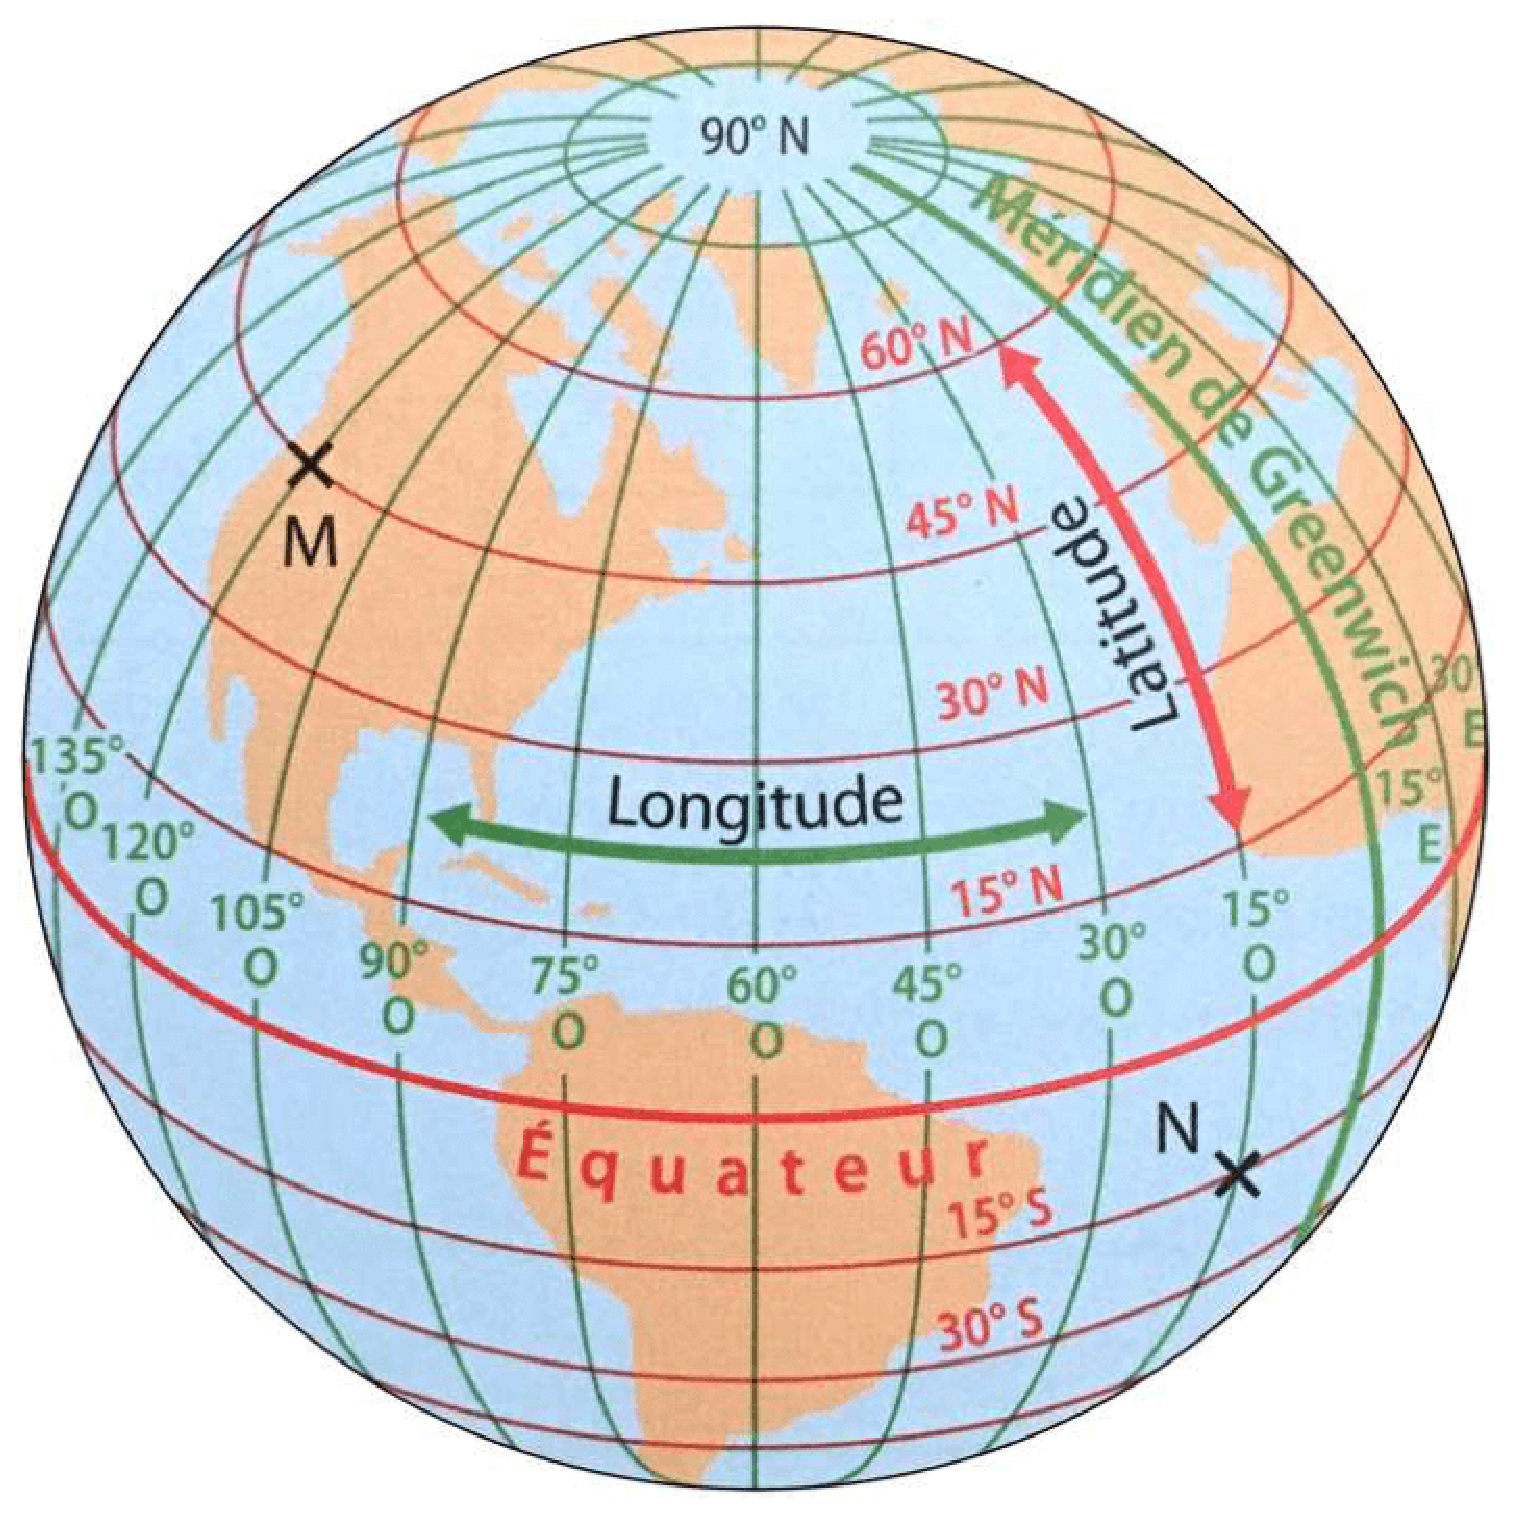
\includegraphics[width=3.5cm]{Geometrie/Images/G12_cours_rep_Terre}
   \correction
      La latitude est comprise entre \udeg{0} et \udeg{90}, Nord ou Sud. \\
      La longitude est comprise entre \udeg{0} et \udeg{180}, Est ou Ouest. \\ [3mm]
      Le point M a pour longitude \udeg{120} Ouest et \udeg{45} Nord. \\
      Montpellier a pour longitude X $=\udeg{43,6}$ N et Y $=\udeg{3,9}$ E.
\end{exemple}


\exercicesbase %%%%%%%%%%%%

\begin{center}
   {\cursive Maîtriser les bases avec} \href{http://mathenpoche.sesamath.net}{
\includegraphics[width=3cm]{Nombres_et_calculs/Images/mathenpoche}} \\
   \bigskip
   {\hautab{0.85}
   \cursive
   \begin{Ltableau}{0.775\linewidth}{4}{C{1}|C{1}|p{7cm}|p{2.3cm}}
      \hline
      Classe & \texttt{N\degre} & Thème & Dans le cours \\
      \hline
      \textcolor{orange}{\bf 6\up{e}} & \texttt{E7} & Espace & 1. à 3.\\
      \hline
      \textcolor{cyan}{\bf 5\up{e}} & \texttt{D6} & Espace & 2. et 3. \\
      \hline
      \textcolor{violet}{\bf 4\up{e}} & \texttt{D5} & Repérages & 5. \\
      \hline
      & \texttt{D6} & Espace  & 1. à 3. \\
      \hline
      \textcolor{teal}{\bf 3\up{e}} & \texttt{D5} & Repérage & 5. \\
      \hline
      & \texttt{D6} & Espace & 3. \\
      \hline
   \end{Ltableau}}
\end{center}

\bigskip


\begin{exercice}[Le chapeau de clown] %%%1
   Pour le carnaval, Noé veut fabriquer un chapeau de clown conique pour sa poupée. Pour cela, il mesure son tour de tête : \ucm{21}. La génératrice du cône mesure \ucm{10}. Construire le développement du chapeau.
\end{exercice}

\begin{corrige}
   Le chapeau peut être découpé dans un disque de rayon $R =\ucm{10}$, longueur de la génératrice du cône. \\
   De plus, l'arc de cercle du développement doit correspondant à \ucm{21} (tour de tête). \\
   Pour calculer l'angle $\alpha$ de la section, on sait que le périmètre du cercle de rayon $R$ vaut $2\pi R \ucm{} =20 \pi\,\ucm{}$ ce qui correspond à \udeg{360}. Donc, 21 cm correspondent à un angle de $\dfrac{\ucm{21}\times\udeg{360}}{20\pi\,\ucm{}}\approx \udeg{120}$.
   \begin{center}
   {\psset{unit=0.75}
      \begin{pspicture}(-6,-5.5)(6,5.5)
         \pscircle(0,0){5}
         \pswedge[fillstyle=solid,fillcolor=blue!75](0,0){5}{-120}{0}
         \psline{<->}(0,0.2)(5,0.2)
         \rput(2.5,0.5){$R =\ucm{10}$}
         \psarc{<->}(0,0){5.3}{-120}{0}
         \psarc[linecolor=white]{<->}(0,0){0.5}{-120}{0}
         \rput(0.7,-0.7){\white $\alpha =\udeg{120}$}
         \pstextpath{\psarc[linestyle=none](0,0){5.6}{-70}{-30}}{\ucm{21}}
      \end{pspicture}}
   \end{center}   
\end{corrige}

\bigskip


\begin{exercice}[just for fun] %%%2
   Combien y-a-t'il de patrons différents du cube (c'est à dire non superposables) ? Les tracer.
\end{exercice}

\begin{corrige}
   On dit que deux patrons sont différents s'ils ne peuvent pas se superposer, ni par rotation, ni par retournement. On peut, par exemple, trouver tous les patrons comprenant quatre faces à la suites, puis trois, puis deux.
   \begin{center}   
      \og {\bf 4 à la suite} \fg{}: \\
      {\psset{unit=0.6}
         \begin{pspicture}(0,0)(4,4.5) %1
            \facer{0}{0} \facec{1}{0} \facec{1}{1} \facec{1}{2} \facec{1}{3} \facer{2}{0}
         \end{pspicture}
         \begin{pspicture}(0,0)(4,4.5) %2
            \facer{0}{0} \facec{1}{0} \facec{1}{1} \facec{1}{2} \facec{1}{3} \facer{2}{1}
         \end{pspicture}
         \begin{pspicture}(0,0)(4,4.5) %3
            \facer{0}{0} \facec{1}{0} \facec{1}{1} \facec{1}{2} \facec{1}{3} \facer{2}{2}
         \end{pspicture}
         \begin{pspicture}(0,0)(4,4.5) %4
            \facer{0}{0} \facec{1}{0} \facec{1}{1} \facec{1}{2} \facec{1}{3} \facer{2}{3}
\end{pspicture}
         \begin{pspicture}(0,0)(4,4.5) %5
            \facer{0}{1} \facec{1}{0} \facec{1}{1} \facec{1}{2} \facec{1}{3} \facer{2}{1}
         \end{pspicture}
         \begin{pspicture}(0,0)(4,4.5) %6
            \facer{0}{1} \facec{1}{0} \facec{1}{1} \facec{1}{2} \facec{1}{3} \facer{2}{2}
         \end{pspicture}

         \og {\bf 3 à la suite} \fg{}: \hspace*{7cm} \og {\bf 2 à la suite} \fg{}: \\
         \begin{pspicture}(0,0)(4,4.5) %7
            \facec{1}{1} \facec{1}{2} \facec{1}{3} \face{2}{0} \face{2}{1} \facer{0}{3}
         \end{pspicture}
         \begin{pspicture}(0,0)(4,4.5) %8
            \facec{1}{1} \facec{1}{2} \facec{1}{3} \face{2}{0} \face{2}{1} \facer{0}{2}
         \end{pspicture}
         \begin{pspicture}(0,0)(3,4.5) %9
            \facec{1}{1} \facec{1}{2} \facec{1}{3} \face{2}{0} \face{2}{1} \facer{0}{1}
         \end{pspicture}
         \begin{pspicture}(0,0)(4,4) %10
            \facec{1}{1} \facec{1}{2} \facec{1}{3} \face{2}{0} \face{2}{1} \facer{2}{-1}
         \end{pspicture}
         \begin{pspicture}(0,0)(4,3.5) %11
            \facec{0}{0} \facec{1}{0} \face{1}{1} \face{2}{1} \face{2}{2} \face{3}{2}
         \end{pspicture}
      }
   \end{center}
\end{corrige}

\bigskip


\begin{exercice}[CRPE blanc 2018 Réunion] %%%3
%%% macros
   \def\unite{\pspolygon[fillstyle=solid,fillcolor=gray](0,0.3)(0.8,0)(0.8,1)(0,1.3)
      \pspolygon[fillstyle=solid,fillcolor=lightgray](0.8,0)(1.65,0.3)(1.65,1.3)(0.8,1)
      \pspolygon[fillstyle=solid,fillcolor=lightgray](0.8,1)(1.65,1.3)(0.85,1.6)(0,1.3)}
   \def\gros{\pspolygon[fillstyle=solid,fillcolor=gray](0,0.6)(1.6,0)(1.6,2)(0,2.6)
      \pspolygon[fillstyle=solid,fillcolor=lightgray](1.6,0)(3.3,0.6)(3.3,2.6)(1.6,2)
      \pspolygon[fillstyle=solid,fillcolor=lightgray](1.6,2)(3.3,2.6)(1.7,3.2)(0,2.6)}
% énoncé
   Les figures ci-dessous représentent un même solide constitué de l'assemblage de quatre cubes : trois cubes d'arête 2~cm et un cube d'arête 4~cm, vu en perspective et vu de face.
   {\psset{unit=0.9}
   \begin{center}
   \parbox{0.4\linewidth}{
      \begin{pspicture}(1,-0.5)(8,5.5)
         \rput(2.9,0.1){\gros}
         \rput(2.1,2.7){\unite}
         \rput(5.35,0.1){\unite}
         \rput(2.85,0.8){\unite}
         \rput(1.5,2){vue de }
         \rput(1.5,1.6){face}
         \rput(7.8,1){vue de }
         \rput(7.8,0.6){droite}
         \rput(4.6,5.2){vue de}
         \rput(4.6,4.8){dessus}
         \psline[linewidth=2pt]{->}(4.6,4.4)(4.6,3.5)
         \psline[linewidth=2pt]{->}(2.1,2.1)(2.7,2.4)
         \psline[linewidth=2pt]{->}(7.6,1.4)(6.4,2)
      \end{pspicture}}
   \qquad
   \parbox{0.4\linewidth}{
   \psset{unit=0.7cm}
      \begin{pspicture}(-1,-0.5)(8,7.5)
         \rput(4,7.5){vue de face}
         \psframe(0,4)(2,6)
         \psframe(2,0)(6,4)
         \psframe(4,2)(6,4)
         \psframe(6,0)(8,2)
      \end{pspicture}}
   \end{center}
   }
   \begin{enumerate}
      \item Dessiner la vue de droite et la vue de dessus de ce solide en vraie grandeur.
      \item On supprime le petit cube le plus à gauche et celui le plus à droite en regardant de face. \\
      On note P le polyèdre restant.
      \begin{center}
      \parbox{0.3\linewidth}{
      \begin{pspicture}(-1,0)(4,3.7)
         \psline(0,2.6)(0,2)
         \psline(0,1)(0,0.6)(1.6,0)(1.6,1)
         \psline(-0.05,2)(-0.05,1)(0.75,0.7)
         \pspolygon(1.6,0)(3.3,0.6)(3.3,2.6)(1.6,2)(0.75,1.7)(0.75,0.7)(1.6,1)
         \psline(1.6,2)(3.3,2.6)(1.7,3.2)(0,2.6)(0.8,2.3)(-0.05,2)(0.75,1.7)
         \psset{linestyle=dashed}
         \psline(1.7,3.2)(1.7,1.25)(3.3,0.6)
         \psline(0,0.6)(1.7,1.25)
         \psline(0.8,2.3)(0.8,1.3)(1.6,1)
         \psline(0.8,1.3)(-0.05,1)
      \end{pspicture}}
   \qquad
   \parbox{0.6\linewidth}{
      \begin{enumerate}
         \item Les faces d'un polyèdre sont les polygones qui le bordent. \\
         Combien le polyèdre P possède-t-il de faces ?
         \item Dessiner un patron de P à l'échelle 1/2. \\
      \end{enumerate}}
      \end{center}
   \end{enumerate}
\end{exercice}

\begin{corrige}
\ \\ [-5mm]
   \begin{enumerate}
      \item On obtient les deux vues de droite, puis de dessus suivantes : \\ \medskip
         \begin{tabular}{C{6}C{1}C{8}}
            \begin{pspicture}(-2,-0.5)(4,6)
               \psframe(4,4)
               \psframe(2,0)(4,2)
               \psframe(0,4)(2,6)
               \psframe(0,2)(-2,4)
            \end{pspicture}
            & &
            \begin{pspicture}(0,-0.5)(8,6)
               \psframe(0,2)(2,4)
               \psframe(2,2)(6,6)
               \psframe(6,4)(8,6)
               \psframe(4,0)(6,2)
            \end{pspicture} \\
         \end{tabular}
      \item 
      \begin{enumerate}
         \item Le polynôme P possède {\blue 9 faces}. 
         \item Un exemple de patron à l'échelle 1/2 :
            \begin{pspicture}(-4,0)(8,6.7)
               \psframe(0,2)(2,4)
               \psframe(2,0)(4,2)
               \psframe(6,2)(8,4)
               \pspolygon(2,2)(4,2)(4,7)(3,7)(3,6)(2,6)(2,5)(3,5)(3,4)(2,4)
               \psline(4,2)(6,2)
               \psline(4,6)(3,6)(3,5)(5,5)(5,4)(7,4)
               \psline(8,4)(8,6)(7,6)(7,5)(6,5)(6,4)
            \end{pspicture}
      \end{enumerate}
   \end{enumerate}
\end{corrige}

\bigskip


\begin{exercice}[En repérage\dots] %%%4
   Dans le pavé droit suivant, on se place dans le repère orthonormé $(A;AI,AJ,AK)$ dont l'unité sur chaque axe est \ucm{1}. On sait que $AB=\ucm{8}, AE=\ucm{3}$ et $AD=\ucm{5}$.
   \begin{center}
   {\psset{unit=0.6}
      \begin{pspicture}(0,-0.3)(10,7.5)
         \pstGeonode[PosAngle={-90,-90,90,180,-90,-90,90,90,-90,0,180,0}](0,0){A}(8,0){B}(8,5){C}(0,5){D}(2,2){E}(10,2){F}(10,7){G}(2,7){H}(1,0){I}(0.67,0.67){J}(0,1){K}(9,3.5){M}
         \pspolygon(A)(B)(F)(G)(H)(D)
         \psline(D)(C)(G)
         \psline(B)(C)
         \psline[linestyle=dashed](H)(E)(F)
         \psline[linewidth=1.5pt]{<->}(0,6)(A)(9,0)
         \psline[linewidth=1.5pt]{->}(A)(2.6,2.6)
         \psline[linestyle=dotted](B)(G)
         \psline[linestyle=dotted](C)(F)
      \end{pspicture}
   }
   \end{center}
   \begin{enumerate}
      \item Indiquer les coordonnées des chacun des huit sommets du pavé droit.
      \item Indiquer les coordonnées des chacun des douze milieux des arêtes du pavé droit.
      \item $M$ est le centre de la face $(BCGF)$. Indiquer les coordonnées de chacun des six centres des six faces du pavé droit.
   \end{enumerate}
\end{exercice}

\begin{corrige}
\ \\ \vspace*{-9mm}
   \begin{multicols}{3}
   \begin{enumerate}
      \item {\blue
         $A(0\,;\,0\,;\,0)$ \\
         $B(8\,;\,0\,;\,0)$ \\
         $C(8\,;\,0\,;\,5)$ \\
         $D(0\,;\,0\,;\,5)$ \\
         $E(0\,;\,3\,;\,0)$ \\
         $F(8\,;\,3\,;\,0)$ \\
         $G(8\,;\,3\,;\,5)$ \\
         $H(0\,;\,3\,;\,5)$}
         \columnbreak
      \item  {\blue
         Milieu de $[AB]$ : $(4\,;\,0\,;\,0)$.\\
         Milieu de $[BC]$ : $(8\,;\,0\,;\,2,5)$ \\
         Milieu de $[CD]$ : $(4\,;\,0\,;\,5)$ \\
         Milieu de $[DA]$ : $(0\,;\,0\,;\,2,5)$ \\
         Milieu de $[DH]$ : $(0\,;\,1,5\,;\,5)$ \\
         Milieu de $[HG]$ : $(4\,;\,3\,;\,5)$ \\
         Milieu de $[GC]$ : $(8\,;\,1,5\,;\,5)$ \\
         Milieu de $[BF]$ : $(8\,;\,1,5\,;\,0)$ \\
         Milieu de $[FG]$ : $(8\,;\,3\,;\,2,5)$ \\
         Milieu de $[EF]$ : $(4\,;\,3\,;\,0)$ \\
         Milieu de $[EH]$ : $(0\,;\,3\,;\,2,5)$ \\
         Milieu de $[AE]$ : $(0\,;\,1,5\,;\,0)$}
         \columnbreak
      \item  {\blue
         Centre de $(ABCD)$ : $(4\,;\,0\,;\,2,5)$ \\
         Centre de $(CDHG)$ : $(4\,;\,1,5\,;\,5)$ \\
         Centre de $(BCGF)$ : $(8\,;\,1,5\,;\,2,5)$ \\
         Centre de $(AEHD)$ : $(0\,;\,1,5\,;\,2,5)$ \\
         Centre de $(AEFB)$ : $(4\,;\,1,5\,;\,0)$ \\
         Centre de $(EFGH)$ : $(4\,;\,3\,;\,2,5)$}
      \end{enumerate}
   \end{multicols}
\end{corrige}

\bigskip


\begin{exercice}[La relation d'Euler] %%%5
   {\it D'après une activité parue dans la revue {\it Envol}. n129, octobre-novembre-décembre 2004.} \\ [1mm]
   Pour chaque polyèdre nommé dans le tableau, retrouver sa représentation en perspective cavalière page suivante, dénombrer le nombre de sommets S, le nombre d'arêtes A et le nombre de faces F, puis calculer la caractéristique d'Euler S $-$ A + F. \\
   Enfin, dire si le solide est régulier, convexe, et s'il s'agit d'un solide de Platon (polyèdre régulier convexe). Discuter des valeurs obtenues.
   \begin{center}   
      {\hautab{1.8}
      \begin{CLtableau}{0.958\linewidth}{9}{C{3}|C{0.9}|C{0.9}|C{0.9}|C{0.9}|C{1.4}|C{1.4}|C{1.4}|C{1.4}}
         \hline
         Nom du solide & n & S & A & F & S $-$ A + F & régulier ? & convexe ? & Platon ? \\
         \hline
         Tétraèdre & & & & & & & & \\
         \hline
         Polyèdre étoilé & & & & & & & & \\
         \hline
         Octaèdre & & & & & & & & \\
         \hline
         Pyramide & & & & & & & & \\
         \hline
          Icosaèdre & & & & & & & & \\
         \hline
         Prisme & & & & & & & & \\
         \hline
          Cube & & & & & & & & \\
         \hline
         Beignoïde  & & & & & & & & \\
         \hline
         Dodécaèdre & & & & & & & & \\
         \hline    
      \end{CLtableau}
   }
   \end{center}

{\psset{unit=0.9}
\begin{pspicture}(-4,-6)(18,18)
   \rput(12,16){\psSolid[object=cube,a=1,RotZ=20,action=draw*, fillcolor=orange!20] \\ {\Huge2}}
   \rput(6,-4){\psSolid[object=tetrahedron,r=1.1,RotZ=20,action=draw*,fillcolor=A1!20] \\ {\Huge9}}
   \rput(12,0){\psSolid[object=dodecahedron,a=0.9,RotZ=0,action=draw*,fillcolor=B2!20] \\ {\Huge8}}
   \rput(0,8){\psSolid[object=octahedron,a=1,RotZ=20,action=draw*,fillcolor=yellow!20] \\ {\Huge4}}
   \rput(6,4){\psSolid[object=icosahedron,a=1,RotZ=60,action=draw*,fillcolor=lightgray!20] \\ {\Huge6}}
   \rput(12,7.7){\psSolid[object=prisme,h=0.6,RotZ=10,action=draw*,fillcolor=green!20] \\ {\Huge5}}
   \rput(0,17){\psSolid[object=new, sommets=
   0 -0.7 0 %0
   -0.7 0 0 %1
   0 1 0 %2
   1 0 0 %3
   0 0 -2, %4
  faces={
     [3 2 1 0]
     [4 0 3]
     [4 3 2]
     [4 2 1]
     [4 1 0]},RotZ=40,action=draw*,fillcolor=magenta!20] {\Huge 1}}
   \rput(5.5,12){\psSolid[object=anneau,r=0.4,R=1,h=1.5,ngrid=4,RotZ=30,RotY=50,action=draw*,fillcolor=cyan!20] \\ {\Huge 3}}
   \rput(0,0){\psSolid[object=new,sommets=
   -0.3 -0.3 -0.3 %0
   0.3 -0.3 -0.3 %1
   0.3 0.3 -0.3 %2
   -0.3 0.3 -0.3 %3
   -0.3 -0.3 0.3 %4
   0.3 -0.3 0.3 %5
   0.3 0.3 0.3 %6
   -0.3 0.3 0.3 %7
   1.5 0 0 %8
   0 1.5 0 %9
   0 0 1.5 %10
   0 0 -1.5 %11
   -1.5 0 0 %12
   0 -1.5 0, %13
   faces={
     [1 2 6 5]
     [0 3 2 1]
     [4 5 6 7]
     [0 1 5 4]
     [3 7 6 2] 
     [0 4 7 3]
     [11 3 2]
     [11 0 3]
     [11 1 0]
     [11 2 1]
     [12 7 3]
     [12 4 7]
     [12 0 4]
     [12 3 0]
     [13 1 5]
     [13 0 1]
     [13 4 0]
     [13 5 4]
     [8 2 6]
     [8 6 5]
     [8 5 1]
     [8 1 2]
     [9 3 7]
     [9 7 6]
     [9 6 2]
     [9 2 3]
     [10 6 7]
     [10 5 6]
     [10 7 4]
     [10 4 5]
     },RotZ=20,RotX=10,action=draw*,fillcolor=vert!20] \\ {\Huge7}}
\end{pspicture}}
\end{exercice}

\begin{corrige}
   Tableau :
   \begin{center}   
      {\hautab{1.8}
      \begin{CLtableau}{0.996\linewidth}{9}{C{3}|C{0.9}|C{0.9}|C{0.9}|C{0.9}|C{1.4}|C{1.4}|C{1.4}|C{1.4}}
         \hline
         Nom du solide & n & S & A & F & S $-$ A + F & régulier ? & convexe ? & Platon ? \\
         \hline
         Tétraèdre & \textcolor{blue}{9} & \textcolor{blue}{4} & \textcolor{blue}{6} & \textcolor{blue}{4} & \textcolor{blue}{2} & \textcolor{blue}{oui} & \textcolor{blue}{oui} &  \textcolor{blue}{oui} \\
         \hline
         Polyèdre étoilé & \textcolor{blue}{7} & \textcolor{blue}{14} & \textcolor{blue}{36} & \textcolor{blue}{24} & 2 & \textcolor{blue}{non} & \textcolor{blue}{non} & \textcolor{blue}{non} \\
         \hline
         Octaèdre & \textcolor{blue}{4} & \textcolor{blue}{6} & \textcolor{blue}{12} & \textcolor{blue}{8} & \textcolor{blue}{2} & \textcolor{blue}{oui} & \textcolor{blue}{oui} & \textcolor{blue}{oui} \\
         \hline
         Pyramide & \textcolor{blue}{1} & \textcolor{blue}{5} & \textcolor{blue}{8} & \textcolor{blue}{5} & \textcolor{blue}{2} & \textcolor{blue}{non} & \textcolor{blue}{oui} & \textcolor{blue}{non} \\
         \hline
          Icosaèdre & \textcolor{blue}{6} & \textcolor{blue}{12} & \textcolor{blue}{30} & \textcolor{blue}{20} & \textcolor{blue}{2} & \textcolor{blue}{oui} & \textcolor{blue}{oui} & \textcolor{blue}{oui} \\
         \hline
         Prisme & \textcolor{blue}{5} & \textcolor{blue}{6} & \textcolor{blue}{9} & \textcolor{blue}{5} & \textcolor{blue}{2} & \textcolor{blue}{non} & \textcolor{blue}{oui} & \textcolor{blue}{non} \\
         \hline
          Cube & \textcolor{blue}{2} & \textcolor{blue}{8} & \textcolor{blue}{12} & \textcolor{blue}{6} & \textcolor{blue}{2} & \textcolor{blue}{oui} & \textcolor{blue}{oui} & \textcolor{blue}{oui} \\
         \hline
         Beignoïde & \textcolor{blue}{3} & \textcolor{blue}{16} & \textcolor{blue}{32} &  \textcolor{blue}{16} & \textcolor{blue}{0} & \textcolor{blue}{non} & \textcolor{blue}{non} & \textcolor{blue}{non} \\
         \hline
         Dodécaèdre & \textcolor{blue}{8} & \textcolor{blue}{20} & \textcolor{blue}{30} & \textcolor{blue}{12} & 2 & \textcolor{blue}{oui} & \textcolor{blue}{oui} & \textcolor{blue}{oui} \\
         \hline    
      \end{CLtableau}}
   \end{center}
\end{corrige}

\bigskip


\begin{exercice}[CRPE 1992 Orléans-Tours] %%%6
%%% macros
   \newcommand{\corte}{\pspolygon[fillstyle=solid,fillcolor=white](0,0)(0.9,0)(0.45,1.7)}
   \newcommand{\boule}{\pscircle[fillstyle=solid,fillcolor=white](0,0.45){0.45}}
   \newcommand{\cube}{\psframe[fillstyle=solid,fillcolor=white](0,0)(1.15,0.9)\psline(0.75,0)(0.75,0.9)}
   \newcommand{\cubeg}{\psframe[fillstyle=solid,fillcolor=white](0,0)(1.15,0.9)\psline(0.4,0)(0.4,0.9)}
%%% énoncé
   On dispose de trois objets sur une table : un cône, un cube et une sphère. On a également des représentations de ces solides selon des points de vue différents : \\
   \hspace*{16mm} {\it Vue de la table du dessus} \hspace{52mm} {\it Solides en vue du dessus et de face}
   \begin{center}
      \begin{pspicture}(-2,-2)(2,2)
         \psframe(-1.5,-1.5)(1.5,1.5)
         \rput(2,2){NE}
         \rput(1.7,1.7){$\swarrow$}
         \rput(2,0){E}
         \rput(1.7,0){$\leftarrow$}
         \rput(2,-2){SE}
         \rput(1.7,-1.7){$\nwarrow$}
         \rput(0,-2){S}
         \rput(0,-1.7){$\uparrow$}
         \rput(-2,-2){SO}
         \rput(-1.7,-1.7){$\nearrow$}
         \rput(-2,0){O}
         \rput(-1.7,0){$\rightarrow$}
         \rput(-2,2){NO}
         \rput(-1.7,1.7){$\searrow$}
         \rput(0,2){N}
         \rput(0,1.7){$\downarrow$}
         \pscircle(0.6,-0.85){0.45}
         \pscircle(-0.25,0.85){0.45}
         \pscircle(-0.25,0.85){0.05}
         \pspolygon(-1,-0.4)(-0.55,0.35)(0.2,-0.1)(-0.25,-0.85)
      \end{pspicture}
      \begin{pspicture}(-2,-2)(8,1.5)
          \rput[l](0.5,1){vue aérienne}
          \pscircle(3.5,1){0.45}
          \pscircle(3.5,1){0.05}
          \pscircle(5.25,1){0.45}
          \rput(7.4,1.25){\pspolygon(-1,-0.4)(-0.55,0.35)(0.2,-0.1)(-0.25,-0.85)}
          \rput[l](0.5,-0.5){vue frontale}
          \rput(3.05,-1.3){\corte}
          \rput(5.25,-.95){\boule}
          \rput(6.4,-0.95){\cube}
      \end{pspicture}
   \end{center} 
   Les images ci-dessous représentent des vues, selon divers axes de visée. Déterminer le point de vue de chaque image (attention, certaines images correspondent à aucune configuration !). \\ [2mm]
   {\hautab{1.5}
   \begin{ltableau}{\linewidth}{8}
      \hline
      N & NE & E & SE & S & SO & O & NO \\
      \hline
      & & & & & & & \\
      \hline
   \end{ltableau}}   
   \begin{center}
      \begin{pspicture}(0,0)(3.3,2.5)
         \psframe(0,0)(3.2,2.5)
         \rput(2.9,2.2){A}
         \rput(0.9,0.2){\boule}
         \rput(1.35,0.2){\cube}
         \rput(1.35,0.2){\corte}
      \end{pspicture}
      \begin{pspicture}(0,0)(3.3,2.5)
         \psframe(0,0)(3.2,2.5)
         \rput(2.9,2.2){B}
         \rput(0.2,0.2){\corte}
         \rput(2.3,0.2){\boule}
         \rput(1.1,0.2){\cube} 
      \end{pspicture}
      \begin{pspicture}(0,0)(3.3,2.5)
         \psframe(0,0)(3.2,2.5)
         \rput(2.9,2.2){C}
         \rput(2.15,0.2){\boule}
         \rput(0.8,0.2){\corte}
         \rput(0.55,0.2){\cube}      
      \end{pspicture}
      \begin{pspicture}(0,0)(3.3,2.5)
         \psframe(0,0)(3.2,2.5)
         \rput(2.9,2.2){D}
         \rput(1.4,0.2){\cube}  
         \rput(0.4,0.2){\corte}
         \rput(0.85,0.2){\boule}
      \end{pspicture}
      \begin{pspicture}(0,0)(3.3,2.5)
         \psframe(0,0)(3.2,2.5)
         \rput(2.9,2.2){E}
         \rput(0.65,0.2){\cube}
         \rput(0.75,0.2){\boule}
         \rput(1.9,0.2){\corte}
      \end{pspicture} \\
      \begin{pspicture}(0,0)(3.3,2.7)
         \psframe(0,0)(3.2,2.5)
         \rput(2.9,2.2){F}
         \rput(1.6,0.2){\boule}
         \rput(1.3,0.2){\cubeg}
         \rput(0.5,0.2){\corte}
      \end{pspicture}
      \begin{pspicture}(0,0)(3.3,2.7)
         \psframe(0,0)(3.2,2.5)
         \rput(2.9,2.2){G}
         \rput(0.3,0.2){\corte}
         \rput(2.55,0.2){\boule}
         \rput(0.8,0.2){\cubeg} 
      \end{pspicture}
      \begin{pspicture}(0,0)(3.3,2.7)
         \psframe(0,0)(3.2,2.5)
         \rput(2.9,2.2){H}
         \rput(0.6,0.2){\corte}
         \rput(1.4,0.2){\cubeg}
         \rput(1.6,0.2){\boule}   
      \end{pspicture}
      \begin{pspicture}(0,0)(3.3,2.7)
         \psframe(0,0)(3.2,2.5)
         \rput(2.9,2.2){I}
         \rput(1.6,0.2){\corte}
         \rput(0.6,0.2){\cubeg}  
        \rput(1.5,0.2){\boule}
      \end{pspicture}
      \begin{pspicture}(0,0)(3.3,2.7)
         \psframe(0,0)(3.2,2.5)
         \rput(2.9,2.2){J}
         \rput(1.2,0.2){\cubeg}
         \rput(0.65,0.2){\boule}
         \rput(2,0.2){\corte}
      \end{pspicture}
   \end{center}
\end{exercice}   

\begin{corrige}
   Les images D et H ne sont pas utilisées. \\ \medskip
   \small
   \hautab{1.5}
   \begin{ltableau}{0.9\linewidth}{8}
      \hline
      N & NE & E & SE & S & SO & O & NO \\
      \hline
      {\blue A} & {\blue J} & {\blue E} & {\blue I} & {\blue C} & {\blue G} & {\blue B} & {\blue F} \\
      \hline
   \end{ltableau}
\end{corrige}  

\bigskip


\begin{exercice}[CRPE 2020 - G4] %%%7
   On donne les coordonnées géographiques, arrondies au degré suivantes :
   \begin{itemize}
      \item de Tahiti : (17° S ; 149° O), soit en écriture anglo-saxonne (S 17°, W 149°) ;
      \item de l’Île de Pâques : (27° S ; 109° O).
   \end{itemize}
   L’Île de Pâques est aussi dénommée, en langue polynésienne, Rapa Nui. Les premiers habitants de l’Île de Pâques étaient originaires de l’Île de Rapa Iti située dans l’archipel des Australes (Polynésie Française). Les coordonnées géographiques de l’Île de Rapa Iti sont (27°S ; 144° O). \\
   
   On souhaite estimer la distance du voyage effectué sur l’Océan Pacifique par ces premiers navigateurs polynésiens. \\
   Estimer la distance entre l’Île de Rapa Iti et l’Île de Rapa Nui en suivant le 27\up{e} parallèle sud, sachant que le rayon du 27\up{e} parallèle sud est environ \ukm{5676}.
\end{exercice}
		
\begin{corrige}
   La situation peut être schématisée en dessinant un arc de cercle pour le 27\up{e} parallèle puisque les îles Rapa Nui et Rapa Iti sont toutes les deux situées sur ce parallèle.
   \begin{center}			
      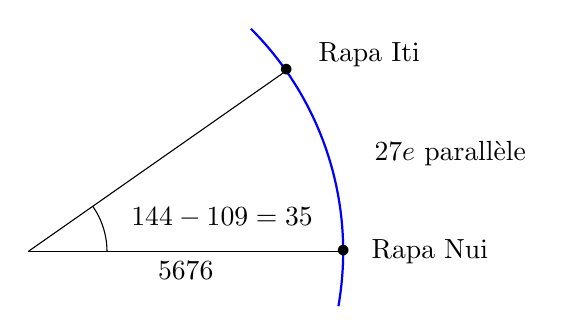
\begin{tikzpicture}
         \draw[blue, thick][samples=100,domain=-10:{144-109+10}] plot({4*cos(\x)},{4*sin(\x)}) ;
         \draw({5.5*cos(13)},{5.5*sin(13)}) node{\blue $27\up{e}$ parallèle};
         \draw (4,0) -- (0,0) node[midway, below]{$\ukm{5676}$};
         \draw (0,0) -- ({4*cos(35)},{4*sin(35)});
         \draw (5.1,0)node{Rapa Nui};
	   \draw (4,0)node{$\bullet$};
         \draw  ({5*cos(30)},{5*sin(30)}) node{Rapa Iti};
         \draw  ({4*cos(35)},{4*sin(35)}) node{$\bullet$};
         \draw [samples=100,domain=0:{35}] plot({1*cos(\x)},{1*sin(\x)}) ;
         \draw ({2.5*cos(10)},{2.5*sin(10)}) node {$\udeg{144}-\udeg{109} =\udeg{35}$};
      \end{tikzpicture}			
   \end{center}		
   La distance entre les deux îles représente une proportion de $\dfrac{35}{360}$ de la longueur du $27\up{e}$ parallèle qui est un cercle. \\
   Or, ce parallèle a une circonférence de $\ell =2\times\pi\times\ukm{5676} =11\,352\,\pi\,\ukm{}$. \\
   Par conséquent, la distance recherchée $d$ vaut : \\
   $d =\dfrac{35}{360}\times11\,352\,\pi\,\ukm{} \approx \ukm{3467,2711}$ \\					
   {\blue Les premiers navigateurs ont parcouru environ $\ukm{3467}$ entre ces deux îles}.
\end{corrige}

\bigskip


\begin{exercice}[CRPE 1996 Dijon] %%%8
   On considère un parallélépipède rectangle pour lequel AB = 2$u$, BC = 3$u$ et AA' = 4$u$, $u$ étant l'unité de mesure de longueur. 
   \begin{center}
   {\psset{unit=1.2}
   \small
      \begin{pspicture}(0,-0.1)(5,4)
         \pspolygon[fillstyle=solid,fillcolor=lightgray](1,4)(0,3)(4,0)(5,1)
         \pspolygon(0,0)(4,0)(5,1)(5,4)(1,4)(0,3)
         \psline(0,3)(4,3)(4,0)
         \psline(4,3)(5,4)
         \psline[linestyle=dashed](0,0)(1,1)(5,1)
         \psline[linestyle=dashed](1,1)(1,4)
         \rput(0.7,4.3){A}
         \rput(-0.3,3){B}
         \rput(-0.3,0){C}
         \rput(0.7,1){D}
         \rput(5.3,4.3){A'}
         \rput(4.3,3){B'}
         \rput(4.3,0){C'}
         \rput(5.3,1.1){D'}
      \end{pspicture}
   }
   \end{center}   
   On pratique une coupe selon le plan (ABC'D'). On obtient deux prismes identiques nommés ADD'C'CB que nous appellerons $P_1$ et AA'D'C'B'B que nous appellerons $P_2$, et qui ont chacun 5 faces.
   \begin{enumerate}
      \item Nommer et donner la nature géométrique des 5 figures planes qui composent $P_1$.
      \item Dessiner deux patrons différents de ce prisme en prenant 1 cm comme unité. La construction sera réalisée sur papier uni, avec règle graduée, équerre et compas.
   \end{enumerate}
\end{exercice}

\begin{corrige}
\ \\ [-5mm]
   \begin{enumerate}
      \item Le prisme ADD'C'CB est composé de :
      \begin{itemize}
         \item {\blue 2 triangles isométriques BCC' et ADD' rectangles respectivement en C et D} ;
         \item {\blue 3 rectangles ABCD, DCC'D' et ABC'D'}.
      \end{itemize}
      \item On a par exemple, dans le triangle BCC' rectangle en C : CB = \ucm{3} et CC' = \ucm{4}, donc le troisième côté BC' mesure \ucm{5} car (3, 4, 5) est un triplet pythagoricien. \\
      {\psset{unit=0.55}
         \begin{pspicture}(-1,-4)(13,4.5)
            \pstGeonode[CurveType=polygon,PosAngle={135,135,-135,-135}](0,1){D}(3,1){A}(3,-1){B}(0,-1){C}
            \pstGeonode[CurveType=polygon,PointName={D',D,C,C'},PosAngle={45,45,-45,-45}](8,1){E}(12,1){F}(12,-1){G}(8,-1){H}
            \pstGeonode[PointName={D,C},PosAngle={90,-90}](4.8,3.4){I}(4.8,-3.4){J}
            \pspolygon(A)(E)(I)
            \pstRightAngle{A}{I}{E}
            \pspolygon(B)(H)(J)
            \pstRightAngle{B}{J}{H}
            \psframe[fillstyle=solid,fillcolor=lightgray](3,-1)(8,1)
         \end{pspicture}
         \begin{pspicture}(2,-4)(15,4.5)
            \pstGeonode[CurveType=polygon,PosAngle={135,-135,-45,45}](3,1){A}(3,-1){B}(8,-1){C'}(8,1){D'}
            \pstGeonode[CurveType=polygon,PointName={D,A,B,C},PosAngle={90,45,-45,-90}](12,1){E}(15,1){F}(15,-1){G}(12,-1){H}
            \pstGeonode[PointName={D,C},PosAngle={90,-90}](4.8,3.4){I}(4.8,-3.4){J}
            \psline(E)(D')(I)(A)
            \pstRightAngle{A}{I}{D'}
            \psline(H)(C')(J)(B)
            \pstRightAngle{B}{J}{C'}
            \psframe[fillstyle=solid,fillcolor=lightgray](3,-1)(8,1)
         \end{pspicture}
      }
   \end{enumerate}
\end{corrige}

\bigskip


\begin{exercice}[CRPE 2018 G3] %%%9
   Soit ABCDEFGH un cube d’arête 6 cm ({\it figure 1}).
   \begin{enumerate}
      \item Soit I, J et K les milieux respectifs des arêtes [FE], [FG] et [FB]. \\
         Quelle est la nature du triangle IJK ? Justifier.
      \item Montrer que le volume du tétraèdre FIJK est \ucmc{4,5}. On rappelle que le volume d’une pyramide est égal au tiers du produit de l’aire d’une base par la hauteur associée.
      \item Construire, en vraie grandeur, un patron du tétraèdre FIJK. On laissera les traits de construction.
      \item On coupe le cube en suivant le plan (IJK), afin d’ôter le tétraèdre FIJK. On procède de la même façon avec chacun des sept autres sommets du cube. Le solide obtenu après ces différentes coupes s’appelle un \og cuboctaèdre \fg ({\it figure 2}).
      \begin{enumerate}
         \item Calculer le volume de ce cuboctaèdre.
         \item Calculer la longueur totale de ses arêtes. On donnera le résultat arrondi au millimètre. \\
      \end{enumerate}
   \end{enumerate}  
   \begin{minipage}{7cm}
      \begin{pspicture}(-2,-1)(4.5,4.5)
         \pspolygon(0,0)(3,0)(4,1)(4,4)(1,4)(0,3)
         \psline(0,3)(3,3)(4,4)
         \psline(3,0)(3,3)
         \psline[linestyle=dashed](0,0)(1,1)(4,1)
         \psline[linestyle=dashed](1,1)(1,4)
         \psdots(1.5,3)(3.5,3.5)(3,1.5)
         \rput(1.5,2.7){I}
         \rput(3.5,3.1){J}
         \rput(3.3,1.5){K}
         \rput(-0.3,-0.3){A}
         \rput(3.3,-0.3){B}
         \rput(4.3,0.9){C}
         \rput(1.2,0.7){D}
         \rput(-0.3,3.1){E}
         \rput(2.8,3.3){F}
         \rput(4.3,4.3){G}
         \rput(0.7,4.3){H}
         \rput(1.7,-0.8){\it figure 1}
      \end{pspicture}
   \end{minipage}
   \begin{minipage}{10cm}
      \begin{center}
         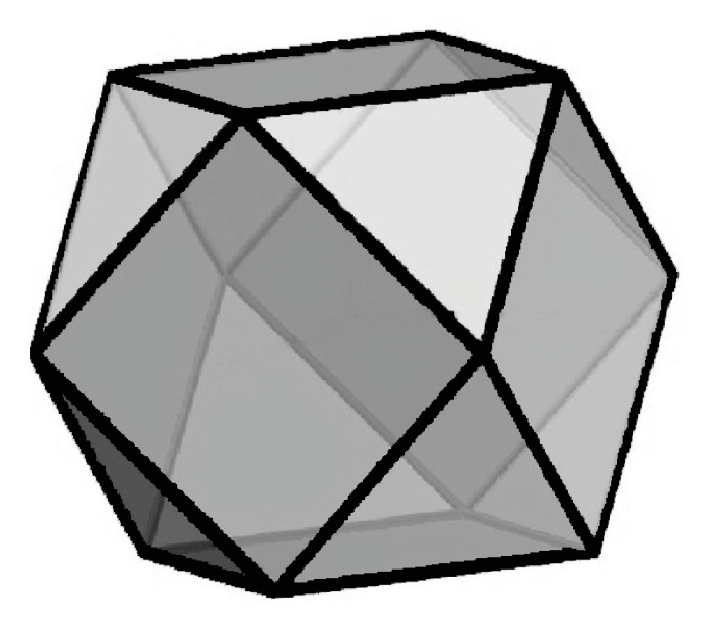
\includegraphics[width=5cm]{Geometrie/Images/G12_ex_cuboctaedre} \\ [3mm]
         {\it figure 2}
      \end{center}
   \end{minipage}
\end{exercice}

\begin{corrige}
\ \\ [-5mm]   
   \begin{enumerate}
      \item I, J et K sont les milieux respectifs des segments [FE], [FG] et [FB] qui sont des arêtes du cube. \\
         On a donc FI = FJ = FK = \ucm{3}. De plus, F est un sommet du cube ce qui signifie que les angles $\widehat{\text{IFK}}, \widehat{\text{KFJ}}$ et $\widehat{\text{JFI}}$ sont droits. Les triangles IFK, KFG et JFI sont donc isométriques et IK = KJ = JI d'où : \\
         {\blue Le triangle IJK est un triangle équilatéral.} \\
      \item On a $V_{\text{tétraèdre}} =\dfrac13\times\mathcal{A}_{\text{FIJ}}\times\text{ FK} =\dfrac13\times\dfrac{\ucm{3}\times\ucm{3}}{2}\times\ucm{3} =\ucmc{4,5}$. \\ [1mm]
         {\blue Le volume du tétraèdre FIJK est de \ucmc{4,5}.} \\
      \item Patron à l'échelle 3/4 : \\
      {\psset{unit=0.75}
         \begin{pspicture}(-6,-0.75)(7.5,6.5)
            \psline(0,3)(6,3)
            \psline(3,6)(3,0)(0,3)(3,6)(6,3)(7.1,7.1)(3,6)
            \rput(3.3,2.7){F}
            \rput(-0.3,3){I}
            \rput(3,-0.3){K}
            \rput(3,6.3){J}
            \rput(6.3,2.7){K}
            \rput(7.4,7.4){I}
            \psframe(3,3)(3.3,3.3)
         \end{pspicture}
      }
      \item On peut démontrer de manière analogue à la question 1. que toutes les arêtes du cuboctaèdre sont de même longueur et donc que tous les tétraèdre ôtés sont isométriques.
         \begin{enumerate}
            \item $\mathcal{V}_{\text{cuboctaèdre}} =\mathcal{V}_{\text{cube}}-8\,\mathcal{V}_{\text{tétraèdre}} =(\ucmc{6})-8\times\ucmc{4,5} =\ucmc{180}$. \\ [1mm]
               {\blue Le volume du cuboctaèdre est de \ucmc{180}}. \\
            \item Le cuboctaèdre possède 3 arêtes à chaque \og coin \fg{} ôté du cube, soit $8\times3$ arêtes = 24 arêtes. \\
               Calculons par exemple IK : dans le triangle IFK rectangle en F, d'après le théorème de Pythagore avec des mesures en centimètre on a $\text{IK}^2 =\text{IF}^2+\text{FK}^2 =3^2+3^2 =18$, donc $\text{IK} =\sqrt{18} =3\sqrt2$. \\
               D'où, la longueur totale des arêtes vaut $24\times3\sqrt2 =72\sqrt2 \approx101,82$ et \\
               {\blue la longueur totale des arêtes du cuboctaèdre vaut environ \ucm{101,8}}.
         \end{enumerate}
   \end{enumerate}
\end{corrige}

\bigskip


\begin{exercice}[CRPE 2015 G2] %%%10
\ \\ [-5mm]
   \begin{minipage}{8.5cm}
      {\it Les différents figures de cet exercice ne sont pas à l'échelle.} \\ [5mm]
      L'objet de ce problème est l'étude d'une pyramide en verre, destinée à être remplie de sable pour constituer un objet de décoration. \\
      Cette pyramide est inscriptible dans un pavé droit, comme indiqué ci-contre. Le pavé droit a pour dimensions : \ucm{9} de longueur, \ucm{9} de largeur et \ucm{12} de hauteur.
   \end{minipage}
   \qquad
   \begin{minipage}{8cm}
   {\psset{unit=1.2}
   \small
      \begin{pspicture}(-1,-0.5)(5.5,5.2)
         \pspolygon[fillstyle=solid,fillcolor=lightgray,linecolor=white](0,0)(3,0)(4.5,1)(1.5,1)
         \pspolygon[fillstyle=solid,fillcolor=lightgray!50,linecolor=lightgray!50](0,0)(1.5,1)(4.5,1)(0,4)
         \pspolygon(0,0)(3,0)(4.5,1)(4.5,5)(1.5,5)(0,4)
         \psline(3,0)(3,4)(0,4)
         \psline(3,4)(4.5,5)
         \psline(3,0)(0,4)(4.5,1)
         \psline[linestyle=dashed](0,0)(1.5,1)(4.5,1)
         \psline[linestyle=dashed](0,4)(1.5,1)(1.4,5)
         \rput(1.5,-0.4){\ucm{9}}
         \rput(4.1,0.25){\ucm{9}}
         \rput(5,3){\ucm{12}}
         \rput(0,-0.3){H}
         \rput(3,-0.3){E}
         \rput(4.5,0.7){F}
         \rput(0,4.3){D}
         \rput(1.5,5.3){C}
         \rput(4.5,5.3){B}
         \rput(3,4.4){A}
         \rput(1.5,0.7){G}
      \end{pspicture}}
   \end{minipage}
   \begin{enumerate}
      \item Réalisation d'un patron de la pyramide.
         \begin{enumerate}
            \item Calculer les longueurs DE et DG.
            \item Quelle est la nature du triangle DGF ? Du triangle DEF ? (on ne demande pas de justification.)
            \item Tracer sur la copie un patron de cette pyramide à l'échelle 1/3.
         \end{enumerate}
   \end{enumerate}
   \begin{minipage}{8.5cm}
      La pyramide est remplie avec du sable de deux couleurs différentes : la partie inférieure avec du sable rouge et la partie supérieure avec du sable blanc. \\
      Sur la figure ci-contre, le point J indique la hauteur à laquelle s'arrête le sable rouge ; les deux couleurs de sable sont délimitées par le plan parallèle à la base de la pyramide DEFGH passant par le point J. \\
      La section est un quadrilatère JKLM où les points K, L, M appartiennent respectivement aux segments [DE], [DF] et [DG]. La pyramide DJKLM est une réduction de la pyramide DEFGH. 
   \end{minipage}
   \qquad
   \begin{minipage}{8cm}
   {\psset{unit=1.2}
   \small
      \begin{pspicture}(-1,-1)(5.5,5)
         \pspolygon[fillstyle=solid,fillcolor=lightgray,linecolor=white](0,0)(3,0)(4.5,1)(1.5,1)
         \pspolygon[fillstyle=solid,fillcolor=lightgray,linestyle=dashed](0,2)(1.5,2)(2.25,2.5)(0.75,2.5)
         \psline(0,2)(1.5,2)(2.25,2.5)
         \psline(3,0)(0,4)(4.5,1)
         \psline(4.5,1)(3,0)(0,0)(0,4)
         \psline[linestyle=dashed](0,0)(1.5,1)(4.5,1)
         \psline[linestyle=dashed](0,4)(1.5,1)
         \rput(0,-0.3){H}
         \rput(3,-0.3){E}
         \rput(4.5,0.7){F}
         \rput(0,4.3){D}
         \rput(1.5,0.7){G}
         \rput(-0.3,2){J}
         \rput(2,1.9){K}
         \rput(2.4,2.7){L}
         \rput(0.4,2.6){M}
      \end{pspicture}}
   \end{minipage}
   \begin{enumerate}
   \setcounter{enumi}{1}
      \item Dans cette partie, on donne JH = 2 cm.
         \begin{enumerate}
            \item Quelle est la nature du quadrilatère JKLM ? Justifier.
            \item Calculer les longueurs JK et JM en justifiant les calculs.
            \item Déterminer le volume $B$ de sable blanc et le volume $R$ de sable rouge contenus dans la pyramide.
         \end{enumerate}
   \end{enumerate}
\end{exercice}

\begin{corrige}
\ \\ [-5mm]
   \begin{enumerate}
      \item 
         \begin{enumerate}
            \item $\bullet$ Calcul de la longueur DE, en cm : nous sommes en présence d'un pavé, donc le triangle DHE est rectangle en H. D'après le théorème de Pythagore, $\text{DE}^2 =\text{DH}^2+\text{HE}^2 =12^2+9^2 =225$, donc : $\text{DE} =15$. \\
               $\bullet$ Calcul de la longueur DG : le triangle DHG rectangle en H est isométrique au triangle DHE rectangle en H donc : {\blue DG = DE = \ucm{15}}.
            \item {\blue Le triangle DGF est rectangle en G et le triangle DEF est rectangle en E.} car l'arête [FG] est perpendiculaire à la face CDHG, elle est alors perpendiculaire à la droite (GD) contenue dans ce plan.
            \item Exemple de patron à l'échelle 1/3 : \\
            {\small
               \begin{pspicture}(-7,-4)(8,7.7)
                  \pspolygon(0,0)(3,0)(3,3)(0,3)
                  \pspolygon(0,0)(-4,0)(0,3)(0,8)(3,3)(8,0)(3,0)(0,-4)
                  \rput(-0.3,-0.3){H}
                  \rput(3.3,-0.3){E}
                  \rput(3.3,3.3){F}
                  \rput(-0.3,3.3){G}
                  \rput(-4.3,0){D}
                  \rput(-0.3,-4){D}
                  \rput(8.3,0){D}
                  \rput(-0.3,8){D}
               \end{pspicture}
            }
         \end{enumerate}
      \setcounter{enumi}{1}
      \item
         \begin{enumerate}
            \item La pyramide DJKLM est une réduction de la pyramide DEFGH. La base de cette dernière étant un carré, il en est de même pour la base de la pyramide réduite. {\blue JKLM est un carré}.
            \item Les longueurs JK et JM sont égales puisque JKLM est un carré. \\ [1mm]
               Calculons le coefficient de réduction de la pyramide : $\dfrac{\text{DJ}}{\text{DH}} =\dfrac{\ucm{12}-\ucm{2}}{\ucm{12}} =\dfrac{10}{12} =\dfrac56$. \\ [1mm]
               Donc, la longueur du côté du carré JKLM mesure : $\dfrac56\times\ucm{9}  =\ucm{7,5}$. On a {\blue JK = JM = \ucm{7,5}}.
            \item Avec des mesures de longueur en cm et des mesures de volumes en \ucmc{}, on a :
               \begin{itemize}
                  \item volume $B$ du sable blanc : $B =\dfrac13\times\text{aire du carré JKLM}\times\text{ hauteur} =\dfrac13\times7,5^2\times10 =187,5$ ;
                  \item volume $V$ de la pyramide DHEFG : c'est un agrandissement de coefficient $\dfrac65$ de la pyramide DJKLM, donc : $V =\left(\dfrac65\right)^3\times B =\dfrac{6^3}{5^3}\times187,5 =324$ ; \smallskip
                  \item volume $R$ du sable rouge : $R =V-B =324-187,5 =136,5$.
            \end{itemize}
            {\blue Le sable blanc occupe un volume de \ucmc{187,5} et le sable rouge \ucmc{136,5}}.
      \end{enumerate}
   \end{enumerate}
\end{corrige}


%\begin{exercice}[Perspective cavalière\dots{} sans cheval ;-)]
%   Terminer la représentation en perspective cavalière des trois pavés suivants : \\ [1mm]
%  {\psset{unit=0.75}
%      \begin{pspicture}(-1,-1)(22,6)
%      \psgrid[subgriddiv=1,gridlabels=0pt,gridcolor=gray](-1,-1)(22,6)
%      \psset{linewidth=0.7mm}
%      \psline(0,0)(2,0)(2,2)(3,3)% cube
%      \psline(5,0)(5,4) % pavé haut
%      \psline(8,4)(10,5)         
%      \psline[linestyle=dashed](7,1)(10,1) 
%      \psline[linestyle=dashed](12,0)(13,2)(21,2) % pavé plat
%      \psline[linestyle=dashed](13,2)(13,4)
%   \end{pspicture}}
%\end{exercice}

%\begin{corrige}
%\ \\ [-5mm]
%  {\psset{unit=0.7}
%      \begin{pspicture}(-1,-1)(22,6.3)
%      \psgrid[subgriddiv=1,gridlabels=0pt,gridcolor=gray](-1,-1)(22,6)
%      \psset{linewidth=0.5mm}
%      \pspolygon(0,0)(2,0)(3,1)(3,3)(1,3)(0,2) % cube
%      \psline(0,2)(2,2)(2,0)
%      \psline(2,2)(3,3)         
%      \psline[linestyle=dashed](0,0)(1,1)(3,1)
%      \psline[linestyle=dashed](1,1)(1,3)
%      \pspolygon(5,0)(8,0)(10,1)(10,5)(7,5)(5,4) % pavé haut
%      \psline(5,4)(8,4)(8,0)
%      \psline(8,4)(10,5)         
%      \psline[linestyle=dashed](5,0)(7,1)(10,1)
%      \psline[linestyle=dashed](7,1)(7,5)
%      \pspolygon(12,0)(20,0)(21,2)(21,4)(13,4)(12,2) % pavé plat
%      \psline(12,2)(20,2)(21,4)
%      \psline(20,2)(20,0)         
%      \psline[linestyle=dashed](12,0)(13,2)(21,2)
%      \psline[linestyle=dashed](13,2)(13,4)
%   \end{pspicture}}
%\end{corrige}


%\begin{exercice}[Illusion]
%Reproduire la figure suivante en perspective isométrique : combien y a-t-il de cubes entiers ? \\ [2mm]
%{\psset{unit=0.5}
%%Cube
%\newcommand{\cube}[2]     
%   {\rput(#1,#2)
%      {\pspolygon[fillstyle=solid,fillcolor=red](0,0)(0,2)(-2,3)(-2,1)
%       \pspolygon[fillstyle=solid,fillcolor=lightgray](0,0)(2,1)(2,3)(0,2)
%       \pspolygon[fillstyle=solid,fillcolor=black](0,2)(2,3)(0,4)(-2,3)
%      }
%   }
%\begin{pspicture*}(-3,5)(30,18)
%   %\psgrid(-3,3)(30,18)
%   %quadrillage
%   \multido{\n=0+2}{15}{\psline[linestyle=dotted](\n,-2)(\n,20)}
%   \multido{\i=-15+2,\n=0+2}{18}{\psline[linestyle=dotted](-1,\i)(29,\n)}
%   \multido{\i=-15+2,\n=0+2}{18}{\psline[linestyle=dotted](-1,\n)(29,\i)} 
%   %pyramide
%   \cube{6}{12.5}
%   \cube{4}{9.5}
%   \cube{2}{6.5}
%   \cube{8}{9.5}
%   \cube{6}{6.5}
%   \cube{10}{6.5} 
%   \pspolygon[fillstyle=solid,fillcolor=black](2,6.5)(4,5.5)(6,6.5)(4,7.5)
%   \pspolygon[fillstyle=solid,fillcolor=black](8,5.5)(10,6.5)(8,7.5)(6,6.5)
%   \pspolygon[fillstyle=solid,fillcolor=red](12,9.5)(12,11.5)(10,12.5)(10,10.5)
%   \pspolygon[fillstyle=solid,fillcolor=red](10,12.5)(10,14.5)(8,15.5)(8,13.5)
%   \pspolygon[fillstyle=solid,fillcolor=lightgray](0,9.5)(2,10.5)(2,12.5)(0,11.5)
%   \pspolygon[fillstyle=solid,fillcolor=lightgray](2,12.5)(4,13.5)(4,15.5)(2,14.5)    
%\end{pspicture*}}
%\end{exercice}

%\begin{corrige}
%   Si on regarde dans le sens classique, on a tendance à voir six cubes entiers alors qu'en retournant la feuille, on à l'impression d'en voir sept. \\
%\end{corrige}


%\begin{exercice}[Patron svp !]
%   On donne le patron d'un dé, compléter les autres patrons du même dé. \\
%   \begin{pspicture}(0,0)(17,4.3)
%      \def\car{\psframe(0,0)(1,1)}
%      \rput(0,3){\car} \rput(1,3){\car} \rput(1,2){\car} \rput(1,1){\car} \rput(2,1){\car} \rput(2,0){\car}
%      \rput{90}(0.5,3.5){\psdice{3}} \rput(1.5,3.5){\psdice{2}} \rput(1.5,2.5){\psdice{6}} \rput(1.5,1.5){\psdice{5}} \rput(2.5,1.5){\psdice{4}} \rput(2.5,0.5){\psdice{1}} %1
%      \rput(4,3){\car} \rput(5,3){\car} \rput(5,2){\car} \rput(6,2){\car} \rput(6,1){\car} \rput(7,1){\car}
%      \rput{90}(4.5,3.5){\psdice{3}} \rput(5.5,2.5){\psdice{1}}
%      %2
%      \rput(9,3){\car} \rput(10,3){\car} \rput(10,2){\car} \rput(11,2){\car} \rput(12,2){\car} \rput(11,1){\car} %3
%      \rput{90}(9.5,3.5){\psdice{6}} \rput(10.5,2.5){\psdice{4}} \rput(11.5,2.5){\psdice{1}}
%      \rput(14,0){\car} \rput(15,0){\car} \rput(16,0){\car} \rput(15,1){\car} \rput(15,2){\car} \rput(15,3){\car}
%      \rput(15.5,2.5){\psdice{5}} \rput(15.5,1.5){\psdice{1}} \rput(16.5,0.5){\psdice{4}}
%      %4
%   \end{pspicture}
%\end{exercice}

%\begin{corrige}
%\ \\ [-5mm]
%\begin{pspicture}(3,0)(17,4.3)
%   \def\car{\psframe(0,0)(1,1)}
%      \rput(4,3){\car} \rput(5,3){\car} \rput(5,2){\car} \rput(6,2){\car} \rput(6,1){\car} \rput(7,1){\car}
%      \rput{90}(4.5,3.5){\psdice{3}} \rput(5.5,3.5){\psdice{5}} \rput(5.5,2.5){\psdice{1}} \rput(6.5,2.5){\psdice{4}} \rput{90}(6.5,1.5){\psdice{2}} \rput{90}(7.5,1.5){\psdice{6}} 
%      %2
%      \rput(9,3){\car} \rput(10,3){\car} \rput(10,2){\car} \rput(11,2){\car} \rput(12,2){\car} \rput(11,1){\car}
%      \rput{90}(9.5,3.5){\psdice{6}} \rput{90}(10.5,3.5){\psdice{2}}  \rput(10.5,2.5){\psdice{4}} \rput(11.5,2.5){\psdice{1}} \rput(12.5,2.5){\psdice{3}} \rput(11.5,1.5){\psdice{5}} %
%      \rput(14,0){\car} \rput(15,0){\car} \rput(16,0){\car} \rput(15,1){\car} \rput(15,2){\car} \rput(15,3){\car}
%      \rput(15.5,3.5){\psdice{6}} \rput(15.5,2.5){\psdice{5}} \rput(15.5,1.5){\psdice{1}} \rput{90}(14.5,0.5){\psdice{3}} \rput(15.5,0.5){\psdice{2}} \rput(16.5,0.5){\psdice{4}}
%      %4
%   \end{pspicture}
%\end{corrige}


%\begin{exercice}[CRPE 2021 - G1]
%\ \\
%\begin{minipage}{10cm}
%ABCDE est une pyramide régulière à base carrée ABCD telle que EO = AC, O étant l’intersection des deux diagonales du carré ABCD. La longueur des côtés du carré ABCD est de 4 cm.
%\begin{enumerate}
%   \item Déterminer la valeur exacte de EO.
%   \item Calculer la valeur exacte de la longueur AE. En déduire que son arrondi au millimètre est de 6,3 cm.
%   \item Tracer un patron de la pyramide ABCDE en vraie grandeur.
%\end{enumerate}
%\end{minipage}
%\qquad
%\begin{minipage}{5cm}
%\begin{pspicture}(0,0)(5,5)
%   \pstGeonode[CurveType =polygon,PointSymbol=none](0,1){A}(3,0){B}(4,2){C}(2,6){E}
%   \pstGeonode(1.8,2){D}
%   \pstLineAB{B}{E}
%   \psset{linestyle=dashed}
%   \pstLineAB{E}{D}
%   \pstLineAB{A}{D}
%   \pstLineAB{D}{C}
%   \pstLineAB{B}{D}
%   \pstLineAB{A}{C}
%   \pstInterLL{A}{C}{B}{D}{O}
%\end{pspicture}
%\end{minipage}
%\end{exercice}

%\begin{corrige}
%Test
%\end{corrige}


%\begin{exercice}[Des triangles dans un cube] %%%%%%%%%%%%%%
%La figure ci-dessous représente un cube. Compléter le tableau. Pour la dernière ligne, on nommera un triangle autre que ceux déjà cités. \\
%\begin{minipage}{7.5cm}
%\begin{pspicture}(-1.5,-0.5)(4.5,4.75)
%   \pspolygon(0,0)(3,0)(4,1)(4,4)(1,4)(0,3)
%   \psline(0,3)(3,3)(4,4)
%   \psline(3,0)(3,3)
%   \psline[linestyle=dashed](0,0)(1,1)(4,1)
%   \psline[linestyle=dashed](1,1)(1,4)
%   \psdot(4,2.5)
%   \rput(4.3,2.8){J}
%   \rput(4,1.75){=}
%   \rput(4,3.25){=}
%   \rput(-0.3,-0.3){A}
%   \rput(3.3,-0.3){B}
%   \rput(4.3,0.7){C}
%   \rput(1.3,0.7){D}
%   \rput(-0.3,3.3){E}
%   \rput(2.7,3.3){F}
%   \rput(4.3,4.3){G}
%   \rput(0.7,4.3){H}
%\end{pspicture}
%\end{minipage}
%\begin{minipage}{8cm}
%{\renewcommand{\arraystretch}{1.2}
%\begin{CLtableau}{1\linewidth}{4}{c}
%   \hline
%   Triangle & Rectangle ? & Isocèle ? & Équilatéral ? \\
%   \hline
%   DJH & & & \\
%   \hline
%   ACG & & & \\
%   \hline
%   AFC & & & \\
%   \hline
%   EHG & & & \\
%   \hline
%   & oui & non & non \\
%   \hline
%\end{CLtableau}}
%\end{minipage}
%\end{exercice}

%\begin{corrige}
%Ci-dessous le tableau complété : \\ [3mm]
%\begin{center}
%{\renewcommand{\arraystretch}{1.5}
%\begin{CLtableau}{1\linewidth}{4}{c}
%   \hline
%   Triangle & Rectangle ? & Isocèle ? & Équilatéral ? \\
%   \hline
%   DJH & non & {\bf oui} & non \\
%   \hline
%   ACG & {\bf oui} & non & non \\
%   \hline
%   AFC & non & oui & {\bf oui} \\
%   \hline
%   EHG & {\bf oui} & {\bf oui} & non \\
%   \hline
%   {\bf JBC} & oui & non & non \\
%   \hline
%\end{CLtableau}}
%\end{center}
%\end{corrige}

